\makeatletter
\def\cl@chapter{}
\makeatother

\documentclass[smallcondensed]{svjour3}

\usepackage{jas_packages} % packages and referencing customization
\usepackage{fix-cm}
\usepackage{jas_tikz_packages}
\tdplotsetmaincoords{60}{125} % view angle in spherical coordinates
% custom macros for AAS paper
% Poincar\'e correct name
\newcommand{\Poincare}{Poincar\'e }

% Bold face for vectors 
\renewcommand{\vec}[1]{\mathbf{#1}} % vec command now makes it boldface
\let\oldhat\hat
\renewcommand{\hat}[1]{\oldhat{\mathbf{#1}}} % using a hat also makes it boldface

% Macros for discrete states to save some time typing
\newcommand{\xk}{\ensuremath{x_k}}
\newcommand{\xkp}{\ensuremath{x_{k+1}}}
\newcommand{\yk}{\ensuremath{y_{k}}}
\newcommand{\ykp}{\ensuremath{y_{k+1}}}

\newcommand{\pxk}{\ensuremath{p_{x_k}}}
\newcommand{\pxkp}{\ensuremath{p_{x_{k+1}}}}
\newcommand{\pyk}{\ensuremath{p_{y_k}}}
\newcommand{\pykp}{\ensuremath{p_{y_{k+1}}}}

\newcommand{\xdotk}{\ensuremath{\dot{x}_{k}}}
\newcommand{\ydotk}{\ensuremath{\dot{x}_{k}}}
\newcommand{\xdotkp}{\ensuremath{\dot{x}_{k+1}}}
\newcommand{\ydotkp}{\ensuremath{\dot{y}_{k+1}}}

\newcommand{\distonek}{\ensuremath{r_{1_k}}}
\newcommand{\distonekp}{\ensuremath{r_{1_{k+1}}}}
\newcommand{\disttwok}{\ensuremath{r_{2_{k}}}}
\newcommand{\disttwokp}{\ensuremath{r_{2_{k+1}}}}

% costate equations of motion (gauss jordan elimination)
\newcommand{\fonex}{\ensuremath{f_{1_x}}}
\newcommand{\ftwox}{\ensuremath{f_{2_x}}}
\newcommand{\fthreex}{\ensuremath{f_{3_x}}}
\newcommand{\ffourx}{\ensuremath{f_{4_x}}}

\newcommand{\foney}{\ensuremath{f_{1_y}}}
\newcommand{\ftwoy}{\ensuremath{f_{2_y}}}
\newcommand{\fthreey}{\ensuremath{f_{3_y}}}
\newcommand{\ffoury}{\ensuremath{f_{4_y}}}

\newcommand{\fonexd}{\ensuremath{f_{1_{\dot x}}}}
\newcommand{\ftwoxd}{\ensuremath{f_{2_{\dot x}}}}
\newcommand{\fthreexd}{\ensuremath{f_{3_{\dot x}}}}
\newcommand{\ffourxd}{\ensuremath{f_{4_{\dot x}}}}

\newcommand{\foneyd}{\ensuremath{f_{1_{\dot y}}}}
\newcommand{\ftwoyd}{\ensuremath{f_{2_{\dot y}}}}
\newcommand{\fthreeyd}{\ensuremath{f_{3_{\dot y}}}}
\newcommand{\ffouryd}{\ensuremath{f_{4_{\dot y}}}} % defines custom macros

\begin{document}


\title{Systematic Design of Optimal Low-Thrust Transfers for the Three-Body Problem
\thanks{This research has been supported in part by NSF under the grants CMMI-1243000 (transferred from 1029551), CMMI-1335008, and CNS-1337722.}
}

\author{Shankar Kulumani \and Taeyoung Lee}  

\institute{S. Kulumani \and T. Lee \at
                Department of Mechanical \& Aerospace Engineering,\\
                George Washington University,\\
                800 22nd St NW, Washington, DC 20052.\\
                \email{skulumani@gwu.edu}\\
                \email{tylee@gwu.edu}
                }

\date{Received: date / Accepted: date}

\maketitle{}        
\begin{abstract}
We develop a computational approach for the design of continuous low thrust transfers in the planar circular restricted three-body problem.
The use of low thrust propulsion allows the spacecraft to depart from the natural dynamics and enables a wider range of transfers.
We generate the reachable set of the spacecraft and use this to determine transfer opportunities, analogous to the intersection of control-free invariant manifolds.
The reachable set is developed on a lower dimensional \Poincare section and used to design transfer trajectories. 
%Computational geometric mechanics allows for the development of variational integrators and a discrete optimal control problem.
This is solved numerically as a discrete optimal control problem using a variational integrator, which preserve the geometric structure of the motion in the three-body problem.
We demonstrate our approach with two numerical simulations of transfers in the Earth-Moon three-body system.
\keywords{First keyword \and Second keyword \and More}
% \PACS{PACS code1 \and PACS code2 \and more}
% \subclass{MSC code1 \and MSC code2 \and more}
\end{abstract}

\section{Introduction}\label{sec:introduction}

%%-------------- Motivation for low thrust orbital transfers

% enables long duration missions with minimized propellant usage since Isp is so high

% Enables different mission scenarios which are not possible through the use of conventional chemical propulsion (high thrust) systems
Designing spacecraft trajectories is a classic and ongoing topic of research.
There has been significant research into the design of orbital transfers for space vehicles.
Optimal expenditure of onboard propellant is critical to allowing a mission to continue for a longer period of time or to enable the launch of a less massive spacecraft.
Electric propulsion systems offer a much greater specific impulse than chemical systems.
As a result, the greatly increased effeciency allows for greater payload mass or extended duration missions.
However, these electric propulsion systems typically have much less thrust than their chemical counterparts and therefore orbital manuevers have a much longer time of flight.
In spite of this drawback, a wide variety of missions, such as communication and deep space probes, have utilized the unique benefits of low thrust electric propulsion to great effect~\cite{choueiri2009}.

% utilizing the combo of small satellite and low thrust propulsion offers new mission scenarios 
With reduced development intervals and decreased launch costs, small satellites have gained increased attention as a cost effective means of scientific and technologic development. 
Furthermore, these cubesats are easily launched as secondary payloads rather than requiring a dedicated launch.
The merger of small satellites with miniature electric propulsion enables inexpensive and responsive missions requiring large changes in orbital energy or extended mission lifespan.
Recent developments in miniature electric propulsion offer the potential for new research opportunities for small spacecraft~\cite{haque2013}.
The advancements in minature electric propulsion allows for greater flexibility in the deployment of cubesats as secondary payloads.
Without the explicit requirement of a dedicated launch trajectory, cubesats are able to exploit a much wider range of possible mission designs~\cite{folta2015}.
With the potential for more demanding missions, even greater importance is placed on the mission design to ensure that optimal trajectories satisfy mission requirements. 
In addition, non-Keplerian orbits and multi-body dynamics have been shown to allow for a much greater range of potential missions at a reduced energy cost~\cite{folta2015,koon2011}.
Future space missions are increasing in complexity and will require new classes of orbits that are not possible via the traditional patched-conic approach~\cite{ross2006,gomez2001}.
Optimally combining the structure of the dynamic environment with low-thrust propulsion systems is vital for future mission success.


% --------------Issues/Challenges of previous work

% use of direct optimal control
% chaotic systems and initial guesses for optimization
% numerical integration accuracy
% preserving dynamical structure

There has been extensive research focused on the optimal control of spacecraft orbital transfers in the three-body problem~\cite{mingotti2011,grebow2011}. 
Inspite of the long history in astrodynamics, a number of difficulties arise when implenting optimal control techniques.
First, the optimal control problem is typically solved using direct methods, which approximate the continuous problem as a parameter optimization problem.
Alternatively, indirect methods apply the calculus of variations to derive the necessary conditions for optimality.
The indirect approach results in a lower dimensioned problem than the direct approach and provides algebraic conditions that guarantee local optimality in contrast to direct methods which result in sub-optimal solutions.
Second, in order to implement any optimization method a sufficiently accurate ``initial guess'' is required.
Frequently, insight into the problem or intuition on the part of the designer is often required to determine initial conditions that will converge to the desired solution due to the inherent nonlinear and chaotic behavior of the three-body system.
Finally, there is no closed form analytical solution for the three-body problem and there are an insufficient number of analytical constants~\cite{szebehely1967}.
As a result numerical methods are often required to investigate solutions to the three body problem.
Conventional Runge-Kutta integration techniques, such as those implemented in~\cite{mingotti2011,grebow2011}, fail to capture the physical laws and geometric properties of the dynamic system.
As a result, these methods suffer from numerical instability and energy drift behaviors which make them ill-suited for the long-term propagation, e.g. on the order of decades to centuries, which is typical of the three-body problem. 

% control-free trajectories in teh three-body problem 
There exists a rich structure in the three-body problem~\cite{koon2011,ross2006}.
Within the three-body problem, a spacecrafts feasible region of motion is constrained by its energy, or Jacobi integral.
It has been shown that there exist multi-dimensional structures, termed invariant manifolds, of constant energy trajectories that span the state space. 
These invariant manifolds, which are associated with the periodic solutions of the three-body dynamics, allow for the spacecraft to traverse vast expanses of the state space with zero energy change. 
However, the results presented are highly case specific and difficult to generalize to arbitrary transfers.
Also, these results are based on control-free trajectories which rely on the underlying structure of the three-body system. 
The addition of low-thrust propulsion offers the potential of reduced transfer transit times and the ability to depart from teh free motion trajectory to allow for increased transfer opportunities.

% objectives of this work

% description of our work - our approach

% concise summary of contributions

%-------------------- OBJECTIVES OF THIS WORK-----------------------------%
% SYSTEMATIC DESIGN TO AVOID DIFFICULTIES IN CHOOSING A GOOD INITIAL GUESS
% CAPTURE LONG TERM EFFECTS OF LOW THRUST ACCURATELY IN NUMERICAL SIMULATION
In this paper, we propose a systematic design method which enables low-thrust transfers in the planar circular restricted three-body problem.
Utilizing the planar assumption greatly simplifies the problem and allows for the use of established methods in determining periodic orbits and \Poincare~sections.
We utilize the concept of the reachability set to enable a simple methodology of selecting initial conditions to achieve general orbital transfers. 
Through the use of a simple distance metric on a \Poincare~section greatly reduces the dimensionality of the reachability analysis and provides an approximation of the reachability set.
In addition, through the use of geometric integrators we more accurately capture the effects of low thrust on the system dynamics in the numerical simulation over extended periods which are typical of electric propulsion systems. 
With this proposed method, the previous research on control-free trajectories will be generalized with the addition of low thrust propulsion systems.

We defne an optimal control problem to determine the reachability set on a \Poincare~section.
The reachable set, defined as the set of all attainable states subect to the system constraints, allows for the extension of the previous control-free methods based on invariant manifolds.
Defining the reachable set on a \Poincare~section reduces the dimensionality of the system dynamics to the study of a related discrete update map.
While the \Poincare~section is well defined for the planar case, as a 2D representation, it is more challenging to implement and visualize for the general 3D three-body problem.
Instead of relying on intuition or insight into the problem, states are chosen which minimize the distance towards the target on the \Poincare~section.
Through the use of low-thrust control input, the reachable set on the \Poincare~section is enlarged and enables a larger space of potential transfers.
By iteratively computing the reachable set, and minimizing the distance to the target on the \Poincare~section allows for the creation of general transfer trajectories.

In short, the authors present a systematic method of generating optimal transfer orbits in the three-body problem.
Previous results in the design of optimal transfers have relied on suboptimal direct optimization methods and conventional integration techniques.
This paper provides a discrete optimal control formulation to generate the reachability set on a \Poincare section.
We derive and solve the Euler-Lagrange equations to generate the necessary conditions for an optimal solution.
This results in an optimal solution rather than the suboptimal solution typical of direct optimal control methods.
In addition, the use of a geometric integrators ensures numerical stability for long-duration orbit transfers and maintains this behavior with the addition of small magnitude control inputs.
Our computation of the reachable set allows for a simple metric of defining optimal trajectories.
We avoid the issues inherent in selecting a valid initial condition for optimization.
Rather, we choose a state on the reachability set which minimizes the distance toward the desired target.
We demonstrate these capabilities via two numerical examples simulating transfer trajectories in the Earth-Moon system.

\section{Problem Formulation and Mathematical Background}\label{sec:background}

% discuss some of the pros/cons of using PCRTBP model
We utilize the planar circular restricted three body problem~(PCRTBP) as the basis of our system definition. 
It is a popular model in the preliminary analysis of multibody spacecraft trajectories. 
In the context of Earth based mission, the PCRTBP affords a relatively simple dynamic model while still capturing the major third body perturbation of the Moon.
In addition, this model allows for a systematic process to define and exploit \Poincare sections.
Furthermore, the 2D solutions afforded by the PCRTBP are frequently use to gain a qualitative understanding of the trade space of transfers in the Earth-Moon system.
The PCRTBP approach offers insight into the fundamental dynamical structure while capturing the major dynamic properties of the planar motion.
As a result, this approach is best suited for trajectories which do not require large plane changes.

The research in this work utilizes a variety of disparate concepts in dynamics, control theory, and astrodynamics. 
As a result, we briefly present some key concepts in the system model as well as established tools in the three body problem, such as invariant manifolds and \Poincare sections.
In addition, we summarize the derivation of a variational integrator for the PCRTBP which is used in the subsequent geometric optimal control formulation.
\subsection{Planar Circular Restricted Three Body Problem}\label{sec:pcrtbp}
The Earth is assumed to be the more massive primary, \( m_1 \), while the Moon is the second, smaller primary \( m_2\).
The equations of motion are developed in a rotating reference frame which allows for much greater insight into the structure of the dynamics.
Following convention, the system is also non-dimensionalized by the characteristic units of length, mass, and time~\cite{koon2011}.
As a result, the system can be characterized by a single mass ratio parameter \( \mu \),
\begin{equation}
        \mu = \frac{m_2}{m_1+m_2} \, .
        \label{eq:mass_param}
\end{equation}
In the rotating reference frame the Lagrangian is given by
\begin{equation}\label{eq:lagrangian}
    L = \frac{1}{2} \parenth{\parenth{\dot{x} - y}^2 + \parenth{\dot{y} + x}^2} + \frac{1 - \mu}{r_1} + \frac{\mu}{r_2},
\end{equation}
where the distances \( r_1, r_2 \in \R \) define the distance from the spacecraft to each primary and are defined as
\begin{align}
    r_1 &= \sqrt{\parenth{x + \mu}^2 + y^2} , \\
    r_2 &= \sqrt{\parenth{x -1 + \mu}^2 + y^2} .
\end{align}
Following a straightforward application of the Euler-Lagrange equations, a more detailed derivation is provided in~\cite{szebehely1967}, results in the following equations of motion defined in the rotating reference frame
\begin{equation}\label{eqn:cont_dyn}
        \left[\begin{array}{c} \dot{\vecbf{r}} \\ \dot{\vecbf{v}} \end{array} \right] = 
        \left[ \begin{array}{c} \vecbf{v} \\ A \vecbf{v} + \nabla U + \vecbf{u} \end{array} \right] = f\left( t,\vecbf{x}, \vecbf{u}\right) \, ,
\end{equation}
where the matrix \( A \) and psuedo gravitational potential gradient \( \nabla U\) are
\begin{align}
    A &= \left[ \begin{array}{ccc} 0 & 2 & 0 \\ -2 & 0 & 0 \\ 0 & 0 & 0 \end{array} \right], \label{eq:A_mat} \\
    \nabla U &= \left[ \begin{array}{c} x - \frac{ \left(1 - \mu\right) \left(x + \mu\right)}{r_1^3} - \frac{\mu \left( x - 1 + \mu \right)}{r_2^3} \\
                                                                                        y - \frac{ \left(1 - \mu\right) y}{r_1^3} - \frac{\mu y}{r_2^3} \\
                                                                                        - \frac{ \left(1 - \mu\right) z}{r_1^3} - \frac{\mu z}{r_2^3}\end{array}\right]
                                        = \left[\begin{array}{c} U_x \\ U_y \\ U_z\end{array} \right] , \label{eq:grav_pot}
\end{align}
and the control inputs is defined as \( \vecbf{u} = \begin{bmatrix} u_x & u_y \end{bmatrix}^T \in \R^{2\times1} \) and assumed to be continuously variable but bounded in magnitude, i.e. \( \vecbf{u}^T \vecbf{u} \leq u_{max}^2 \).
The state is defined as \( \vecbf{x} = \begin{bmatrix}\vecbf{r} &\vecbf{v} \end{bmatrix}^T\) with \(\vecbf{r} = \begin{bmatrix} x & y \end{bmatrix}^T \in \R^{2\times1}\) and \(\vecbf{v}= \begin{bmatrix} \dot{x} & \dot{y} \end{bmatrix}^T \in \R^{2\times1}\) representing the position and velocity with respect to the system barycenter, respectively.



\subsubsection{Jacobi Integral}\label{sec:jacobi}
There exists a single integral, or constant of motion for the three-body problem~\cite{szebehely1967,lanczos1970}.
This energy constant is analogous to the total mechanical energy, however it is a non-physical quantity arising from the problem formulation~\cite{szebehely1967}.
Also known as the Jacobi constant, it is defined as a function of the position and velocity in the rotating frame and given by
\begin{equation}
        E\left( \vecbf{r} , \vecbf{v} \right) = \frac{1}{2}\left( \dot{x}^2 + \dot{y}^2\right) - U\left(x,y \right) \, .
        \label{eq:jacobi}
\end{equation}
\Cref{eq:jacobi} divides the phase space into distinct regions of allowable motion based on the energy level of the spacecraft.
Fixing the Jacobi integral to a constant defines zero velocity curves, which are the locus of points where the kinetic energy, and hence velocity vanishes.
As seen in Figure~\ref{fig:energy_contour}, the phase space is divided into distinct realms based on the energy level.
In the vicinity of \( m_1\) or \(m_2\) there exists a potential well. 
As the energy level increases there are five critical points of the effective potential where the slope is zero.
Three collinear saddle points on the \(\hat{e}_1\) axis and two equilateral points.
These equilibrium, or Lagrange points, are labeled \( L_i, i = 1, \hdots, 5 \) and are shown in Figure~\ref{fig:energy_contour}.
The Jacobi integral is a valuable invariant property of the three-body system that allows for greater insight into the motion of the spacecraft.
\begin{figure}[htbp]
        \centering
        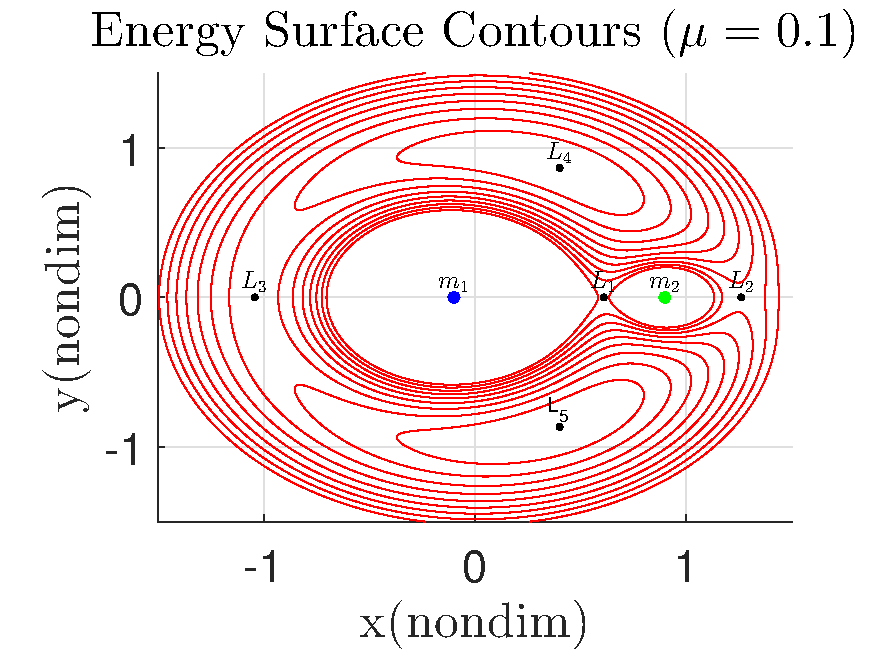
\includegraphics[width=0.5\textwidth]{energy_contours}
        \caption{Contour plot of Jacobi integral}
        \label{fig:energy_contour}
\end{figure} 

\subsubsection{Invariant Manifolds and \Poincare Map}\label{sec:invariant_manifold}
Dynamics systems theory has been applied to the design of control-free manuevers in the restricted three-body problem~\cite{koon2011}.
As previously introduced in~\Cref{sec:jacobi}, there exist five equilibrium points in the equations of motion for the three-body problem.
It has been shown that the local orbit structure near the Lagrange points gives rise to families of periodic orbits as well as the stable and unstable manifolds of these periodic orbits.
This rich structure is globally connected and gives rise to a dynamical chain which allows trajectories to pass through the phase space~\cite{koon2011,conley1968}.
The manifold structure associated with periodic orbits about the \( L_1 \) and \( L_2 \) Lagrange points are critical to the understanding of the motion of spacecraft as well as comets/asteroids.
In addition, the stable and unstable manifolds serve as the boundaries of the phase space region that allow for the transport between realms in a single three-body system or between multiple three-body systems.
These invariant manifolds only exist as a result of the dynamic formulation of the three-body problem in a rotating reference frame. 
Invariant manifolds serve as a higher dimensional generalization of the concept of seperatrices from linear systems as applied to the case of nonlinear systems. 

\Poincare maps are a useful tool in the analysis of the flow near periodic orbits in the three-body problem.
We let \( \Sigma \) define a hypersurface of section chosen such that all trajectories in the vicinity of a state \( \vecbf{q} \in \Sigma \) cross \( \Sigma \) transversely and in the same direction.
A \Poincare map, \( P(\vecbf{q}) = \phi(T;\vecbf{q}) \), maps the state of a trajectory from one intersection to the next.
Choosing a section in this manner results in a \Poincare section as shown in~\cref{fig:poincare_map}.
This allows for greater insight into the stability and dynamics of periodic solutions of a dynamic system as a fixed point on the \Poincare section corresponds to a periodic orbit while movement on the section is associate with the stability of neighboring trajectories. 
For example, \Poincare maps have been used to prove the existence of homoclinic orbits, which are orbits both forward and backward asymptotic to a single unstable periodic orbit, and heteroclinic orbits, which join different periodic orbits~\cite{conley1968,koon2000b}.
These dynamic features have been shown to play a vital role in the movement of natural bodies as well as critical for spacecraft missions~\cite{gomez2001,lo1997}.
\begin{figure}
        \centering
        \begin{scaletikzpicturetowidth}{0.5\textwidth}
    \begin{tikzpicture}[tdplot_main_coords,
      poincare/.style={opacity=.2,very thick,fill=blue},
      orbit/.style={very thick,black},
      orbit hidden/.style={very thick,dashed},
      grid/.style={very thin,gray!50},
      axis/.style={->,blue,thick}, scale=\tikzscale]

    % nodes for the poincare section
    \node[label=above:\(\Sigma\)] (upper_right) at (0,5,5) {};
    \node[] (upper_left) at (0,1,5) {};
    \node[] (lower_left) at (0,1,0) {};
    \node[] (lower_right) at (0,5,0) {};

    % draw poincare section
    \draw[poincare] (upper_right.center) -- (upper_left.center) -- (lower_left.center) -- (lower_right.center) -- (upper_right.center);
    
    % draw a periodic orbit
    \coordinate (center) at (0,0,2);
    \node[below right] (x0) at (0,2,2) {\(\vecbf{q}_0\)};
    \filldraw (0,2,2) circle (3pt);

    \node[below right] (x1) at (0,3,2) {\(\vecbf{q}_1\)};
    \filldraw (0,3,2) circle (3pt);

    \tdplotdrawarc[orbit hidden]{(center)}{2}{90}{190}{}{};
    \tdplotdrawarc[orbit,<-]{(center)}{2}{-170}{90}{}{};

    \tdplotdrawarc[orbit hidden]{(center)}{3}{90}{199}{}{};
    \tdplotdrawarc[orbit,<-]{(center)}{3}{-161}{90}{}{};

        \end{tikzpicture}
    \end{scaletikzpicturetowidth}
        \caption{Diagram of the \Poincare map\label{fig:poincare_map}}
\end{figure}

% drawbacks of this approach on how we seek to improve upon it
Combining invariant manifolds and an appropriate \Poincare section provides a conceptually simple manner to determine trajectories which connect wide regions of the phase space.
However, the results previously developed are highly case specific and difficult to generalize to arbitrary transfers.
Also, these results are based on control-free trajectories which rely on the underlying structure of the three-body system.
In addition, transfer orbits along an invariant manifold require large time of flights which may be undesirable for time critical missions.
The addition of low-thrust propulsion offers the potential of reduced transit times and the ability to depart from the free motion trajectory to allow for increased transfer opportunities. 
In this paper, we formulate an optimal control problem to generate the reachable set of the spacecraft.
We compute the reachable set on an appropriate \Poincare section and use this to design a transfer trajectory.

\subsection{Variational Integrator for PCRTBP}\label{sec:discrete_var}
Geometric numerical integration deals with numerical integration methods which preserve the geometric properties of the flow of a differential equation, such as invaraint properties and symplecticity.
Variational integrators are constructed by discretizing Hamilton's principle rather than the continuous Euler-Lagrange equations.
As a result, integrators developed in this manner have the desirable properties that they are symplectic and momentum preserving.
In addition, they exhibit improved energy behavior over long integration periods.
A thorough discussion of variational integrators is provided in~\cite{west2004,marsden2001}.
We use this approach to construct a variational integrator for the PCRTBP with the inclusion of low-thrust propulsion.

Consider the autonomous mechanical system described by the Lagrangian, \( L(q, \dot{q} ) \), for the generalized coordinates, \( q\) and velocities \( \dot{q} \).
The integration of the continuous Lagrangian along a path, \( q (t) \), followed by the system must satisfy Hamilton's principle, which results in the well-known Euler-Lagrange equations~\cite{lanczos1970}.
In the discrete time scenario, the continuous path \( q(t), \dot{q}(t) \), is replaced by a finite difference approximation over a fixed time step, e.g. \( q_0, \frac{q_1 - q_0}{h} \), which converges to the true velocity as \( h \) tends towards zero.
In this manner, we define a discrete Lagrangian, \( L_d (q_0, q_1, h) \) which approximates the integral of the true Lagrangian over the time interval \( h \) between \( q_0 \) and \( q_1\)~\cite{marsden2001}.

The discrete equations of motion for the PCRTBP are derived by choosing an appropriate quadrature rule to discretize the continuous Lagrangian in~\cref{eq:lagrangian}~\cite{marsden2001}.
In this work, we apply the trapezoidal rule to approximate the action integral over a fixed time interval.
The trapezoidal rule allows for a second order accurate approximation and alleviates the difficulties in applying implicit quadrature schemes.
The discrete Lagrangian for the PCRTBP is given by
\begin{align}\label{eq:discrete_lagrangian}
        L_d = &\frac{h}{2} \left( \frac{1}{2} \bracket{\left(  \frac{\xkp - \xk}{h} -\yk \right)^2 + \left( \frac{\ykp - \yk}{h} + \xk \right)^2} + \frac{1 - \mu}{r_{1_k}} + \frac{\mu}{r_{2_k}} \right. \nonumber \\ 
                & + \left. \frac{1}{2} \bracket{\left(  \frac{\xkp - \xk}{h} -\ykp \right)^2 + \left( \frac{\ykp - \yk}{h} + \xkp \right)^2} + \frac{1-\mu}{r_{1_{k+1}}} + \frac{\mu}{r_{2_{k+1}}}  \right) \, .
\end{align}
Applying a discrete version of the Lagrange-d'Alembert principle allows for inclusion of an external control force on the system~\cite{marsden2001}.
Using~\cref{eq:discrete_lagrangian} and some manipulation, gives the discrete equations of motion as
\begin{subequations}\label{eq:discrete_eoms}
\begin{align}
        \xkp &= \frac{1}{1+ h^2} \bracket{h \dot{x}_k + h^2 \dot{y}_k  + \xk \parenth{1+ \frac{3h^2}{2}} + \frac{h^3}{2} \yk - \frac{h^3}{2} U_{y_k} - \frac{h^2}{2} U_{x_k} } \label{eq:xkp} \, ,\\
        \ykp &= h \dot{y}_k + h \xk - h \xkp + \yk + \frac{h^2 \yk}{2} - \frac{h^2 }{2} U_{y_k} \label{eq:ykp} \, ,\\
        \dot{x}_{k+1} &= \dot{x}_k - 2 \yk + 2 \ykp + \frac{h}{2} \parenth{\xkp + \xk} - \frac{h}{2} U_{\xkp} - \frac{h}{2} U_{\xk} + h u_x \label{eq:xdotkp}\, ,\\
        \dot{y}_{k+1} &= \dot{y}_{k} + 2 \xk - 2 \xkp + \frac{h}{2} \parenth{\ykp + \yk} - \frac{h}{2} U_{\ykp} - \frac{h}{2} U_{\yk} + h u_y \label{eq:ydotkp} \, .
\end{align}
\end{subequations}
The discrete equations of motion are given in the Lagrangian form after applying the discrete fiber derivative as \( p_{\xk} = \dot{x}_k - \yk \) and \( p_{\yk} = \dot{y}_k + \xk \).
The state is defined as \( \vecbf{x}_k = \begin{bmatrix} \xk & \yk & \dot{x}_k & \dot{y}_k \end{bmatrix}^T\) and the control input is \( \vecbf{u} = \begin{bmatrix} u_x & u_y \end{bmatrix}^T \).
This results in a discrete update map \( f_k: \vecbf{x}_k \to \vecbf{x}_{k+1} \) which preserves the same properties of the continuous-time dynamics in~\cref{eqn:cont_dyn} such as invariants, symplecticity, and the configuration manifold.
The discrete potential gradients are given by
\begin{subequations}\label{eq:discrete_potential_grad}
\begin{align}
        U_{\xk} &= \frac{\parenth{1 -\mu} \parenth{\xk + \mu}}{\distonek^3} + \frac{ \mu \parenth{\xk -1 + \mu}}{\disttwok^3} \label{eq:Uxk} \, ,\\
        U_{\yk} &= \frac{\parenth{1 -\mu} \yk}{\disttwok^3} + \frac{ \mu \yk}{\disttwok^3} \label{eq:Uyk} \, ,\\
        U_{\xkp} &= \frac{\parenth{1 -\mu} \parenth{\xkp + \mu}}{\distonekp^3} + \frac{ \mu \parenth{\xkp -1 + \mu}}{\disttwokp^3} \label{eq:Uxkp}\, ,\\
        U_{\ykp} &= \frac{\parenth{1 -\mu} \ykp}{\distonekp^3} + \frac{ \mu \ykp}{\disttwokp^3} \label{eq:Uykp} \, .
\end{align}     
\end{subequations}
The distances to each primary are defined as
\begin{subequations}\label{eq:discrete_distance}
\begin{align}
        \distonek &= \sqrt{\left( \xk + \mu\right)^2 + \yk^2} \label{eq:distonek}\, ,\\
        \disttwok &= \sqrt{\left( \xk - 1 + \mu\right)^2 + \yk^2} \label{eq:disttwok}\, ,\\
        \distonekp &= \sqrt{\left( \xkp + \mu\right)^2 + \ykp^2} \label{eq:distonekp}\, ,\\
        \disttwokp &= \sqrt{\left( \xkp - 1 + \mu\right)^2 + \ykp^2} \label{eq:disttwokp} \, .
\end{align}
\end{subequations}
Care must be taken during the implementation of~\cref{eq:discrete_eoms}.
As~\cref{eq:discrete_potential_grad,eq:discrete_distance} are defined at both step \( k \) and \( k+1 \) they must be evaluated at both time instances.
\Cref{eq:discrete_eoms} is implemented by first defining an initial state \( \vecbf{x}_k \) and control \( \vecbf{u}_k \).
The distances and gravitational potential at step \( k \) are evaluated from~\cref{eq:distonek,eq:disttwok,eq:Uxk,eq:Uyk}.
The discrete update steps in~\cref{eq:xkp,eq:ykp} are evaluated to generate \( \xkp \) and \( \ykp\).
Next, the distances and gravitational potential at step \( k+1 \) are evaluated from~\cref{eq:distonekp,eq:disttwokp,eq:Uxkp,eq:Uykp}. 
Finally, the update steps in~\cref{eq:xdotkp,eq:ydotkp} are evaluated.
This results in the complete discrete update map \( \vecbf{x}_k \to \vecbf{x}_{k+1} \) given \( \vecbf{u}_k \).
\subsection{Numerical Example}\label{sec:variational_example}
\begin{figure} 
        \centering 
        \begin{subfigure}[h]{0.5\textwidth} 
                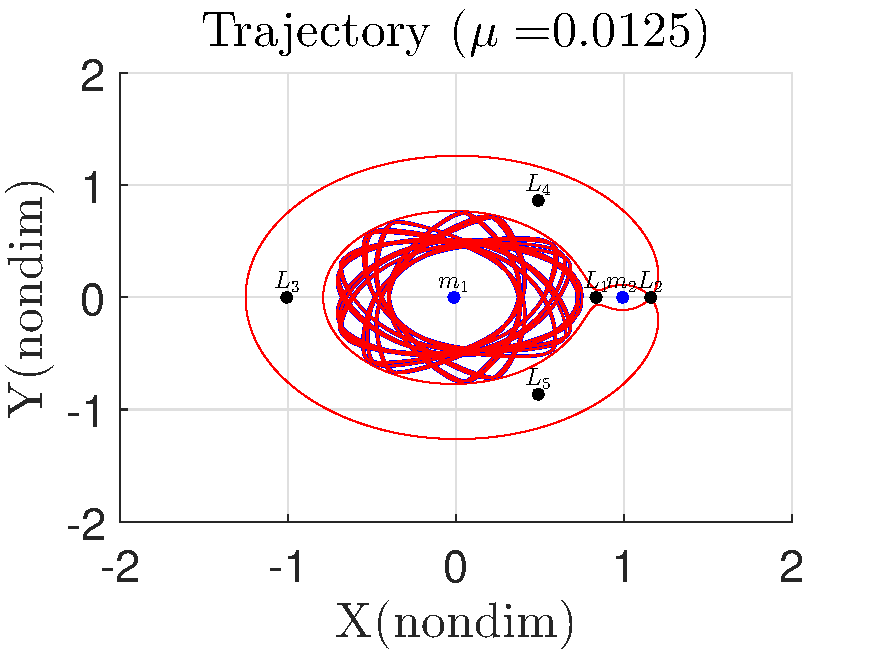
\includegraphics[width=\textwidth]{trajectory} 
                \caption{Earth-Moon three-body trajectory used for integrator comparision} \label{fig:compare_trajectory} 
        \end{subfigure}~ %add desired spacing between images, e. g. ~, \quad, \qquad, \hfill etc. %(or a blank line to force the subfigure onto a new line) 
%       \begin{subfigure}[htbp]{0.3\textwidth} 
%               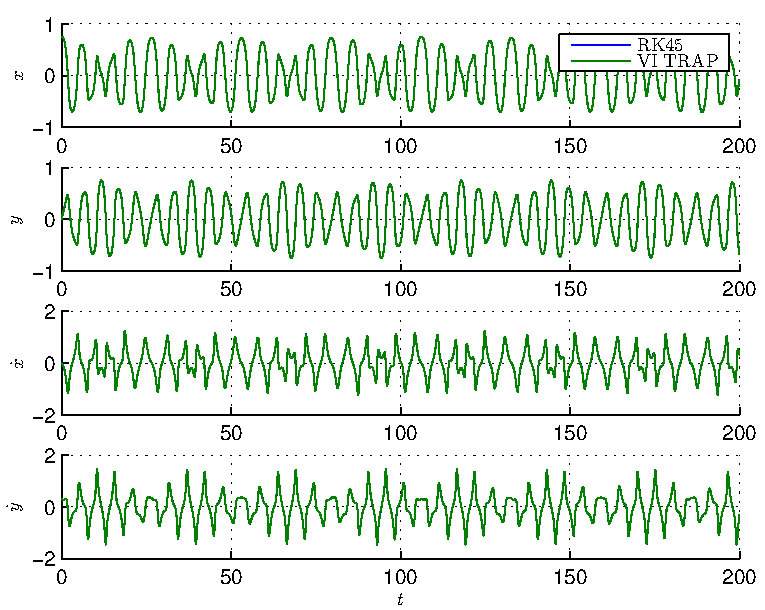
\includegraphics[width=\textwidth]{components} 
%               \caption{State \( \parenth{x , y, \dot{x}, \dot{y}}\)} \label{fig:compare_components} 
%       \end{subfigure} ~ %add desired spacing between images, e. g. ~, \quad, \qquad, \hfill etc. %(or a blank line to force the subfigure onto a new line) 
        \begin{subfigure}[htbp]{0.5\textwidth} 
                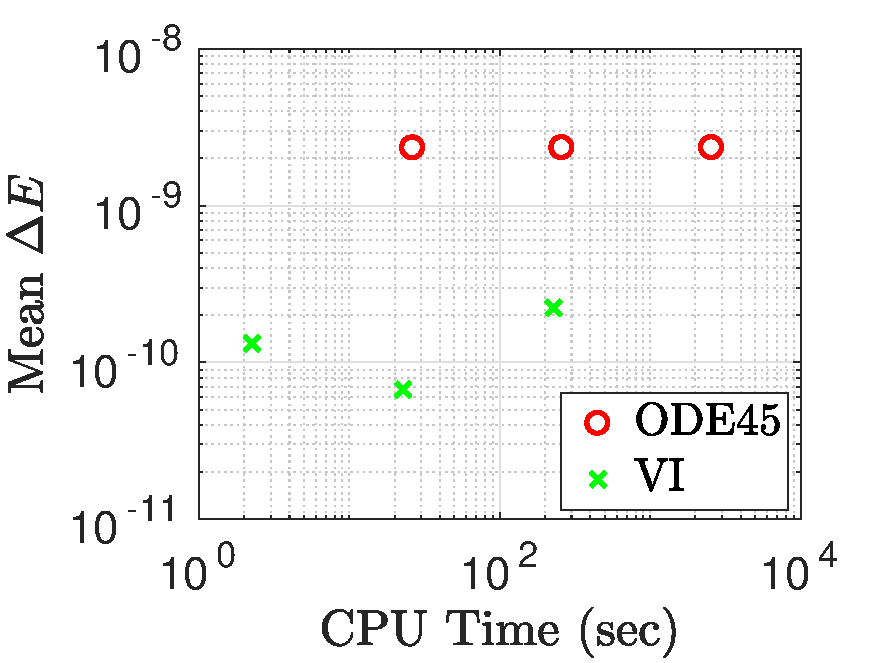
\includegraphics[width=\textwidth]{figures/cputimevsE.pdf} 
                \caption{Mean Jacobi integral deviation between variational integrator and Matlab \texttt{ODE45}} \label{fig:compare_energy} 
        \end{subfigure} 
        \caption{Integrator Comparison}
        \label{fig:integrator_compare} 
\end{figure}
A simulation comparing the variational integrator to a conventional Runge-Kutta method is given in~\cref{fig:integrator_compare}.
A particle is simulated from an initial condition of \( \vecbf{x}_0 = \begin{bmatrix} 0.75 & 0 & 0 & 0.2883\end{bmatrix}^T \) for \( t_f = 200 \approx 15\) years in the Earth-Moon system.
    The variational integrator uses a range of step sizes between \SIrange{4.72}{472}{\second} while the Runge-Kutta method uses a variable step size implemented via \texttt{ODE45} in Matlab.
    The step size of the variable integrator is varied to approximately match the run time required by the conventional \texttt{ODE45} integrator.
\Cref{fig:compare_trajectory} shows the trajectory of the spacecraft in the rotating reference for this comparison.
Both integration schemes result in trajectories that are initially nearly identical.
\Cref{fig:compare_energy} shows the mean Jacobi integral deviation over the entire simulation time as a function of computation time.
For a given computational effort, in the form of simulation run time, the variational integrator will provide a smaller energy deviation as compared to the convential integration scheme.
Over long simulation horizons or with the addition of small control inputs the inability of conventional integration schemes to accurately track the system energy limits the applicability of conventional techniques in which energy conservation is mandatory for characterizing the solution space.

\section{Optimal Control Formulation for Reachability Set}
% introduce method
In this section, an optimal control formulation is presented to determine and design transfers within the three-body problem.
The application of variational integrators to optimal control problems is referred to as computational geometric optimal control.
Our formulation is based on the concept of the reachability set on a \Poincare section.
This method allows one to easily determine potential transfer opportunities by finding set intersections on a lower dimensional space and greatly reduces the design process.
The addition of continuous low thrust propulsion extends the control free design process developed previously and allows for a greater range of potential transfers with a reduced time of flight.

The numerical examples presented in this section are designed in the context of the PCRTBP.
The dynamic environment has a four dimensional state space and offers a convient integration constant in the form of the Jacobi integral.
As a result, there are well defined methods to define and exploit \Poincare sections, which result in straightforward two-dimensional subspaces of the system.
Our approach uses the \Poincare section to approximate the reachability set on this reduced subspace.
As a result, this approach is more difficult to apply to three-dimensional transfers in the general three body problem.
\Poincare sections in the case of the general six dimensional state space are significantly more challenging and typically require more complicated visualization techniques. 
However, this is an area of active research and some of the authors future research is aimed at implementing this approach for non-planar transfer trajectories.

\subsection{Reachability Set}\label{sec:reachability_set}
% discuss reachability and application to space system
Reachability theory provides a framework to evaluate control capability and safety.  
The reachable set contains all possible trajectories that are achievable over a fixed time horizon from a defined initial condition, subject to the operational constraints of the system.
Reachability theory has been applied to aerospace systems such as collision avoidance, safety planning, and performance characterization.
The theory formally supporting reachability has been extensively developed and is directly derivable from optimal control theory~\cite{varaiya2000,lygeros2002,lygeros2004}.
More recently, reachability theory has recently been applied to space systems~\cite{holzinger2009,komendera2012a}.
Computation of the reachable set for a system involves solving the Hamilton-Jacobi partial differential equation or satisfying a dynamic programming principle.
Analytical computation of reachable sets is an ongoing problem and is only possible for certain classes of systems.
Typically, numerical methods are used to generate approximations of the reachability set, but are generally limited by the dimensionality of the problem.
 
Computation of reachable sets is critical to space situational awareness, rendezvous and proximity operations, and orbit determination operations.
Specifically, maintaining accurate estimates of a spacecraft state over extended periods is not trivial.
The challenge is increased for multiple spacecraft operating in close proximity or when there are long periods of time between measurements.
Coupling the ability for continuous low-thrust propulsion between measurements increases the measurement association complexity.
Computing the reachability set given estimated states and control authorities allows one to better correlate subsequent measurements or determine sensor pointing regions in the event of a lost spacecraft. 

\subsection{Optimal Control Formulation}\label{sec:optimal_control}
In this paper, we seek to approximate the reachability set on a \Poincare section by solving a related optimal control problem. 
We choose our \Poincare section in a similar manner to those used previously for the design of transfers via invariant manifolds.
The \Poincare section is chosen to intersect transversally with trajectories emanating from the initial orbit. 
In the case of a periodic orbit the trajectories will cross the \Poincare section at two distinct fixed points every half period.
The main idea is that the addition of low thrust propulsion allows us to enlarge the set of trajectories achievable in the \Poincare section. 
\Cref{fig:reachability_set} illustrates how, without any control input, trajectories will intersect with the \Poincare section at \( \vecbf{x}_n \). 
However, the addition of low thrust propulsion allows the spacecraft to depart from the natural dynamics and intersect the \Poincare section at a different location.
We use a cost function to define a distance metric on the \Poincare section from the control-free intersection to an intersection under the influence of the control input.
Maximization of this distance along varying directions enables us to generate the largest reachability set under the bounded control input.
\begin{figure}
        \centering
%       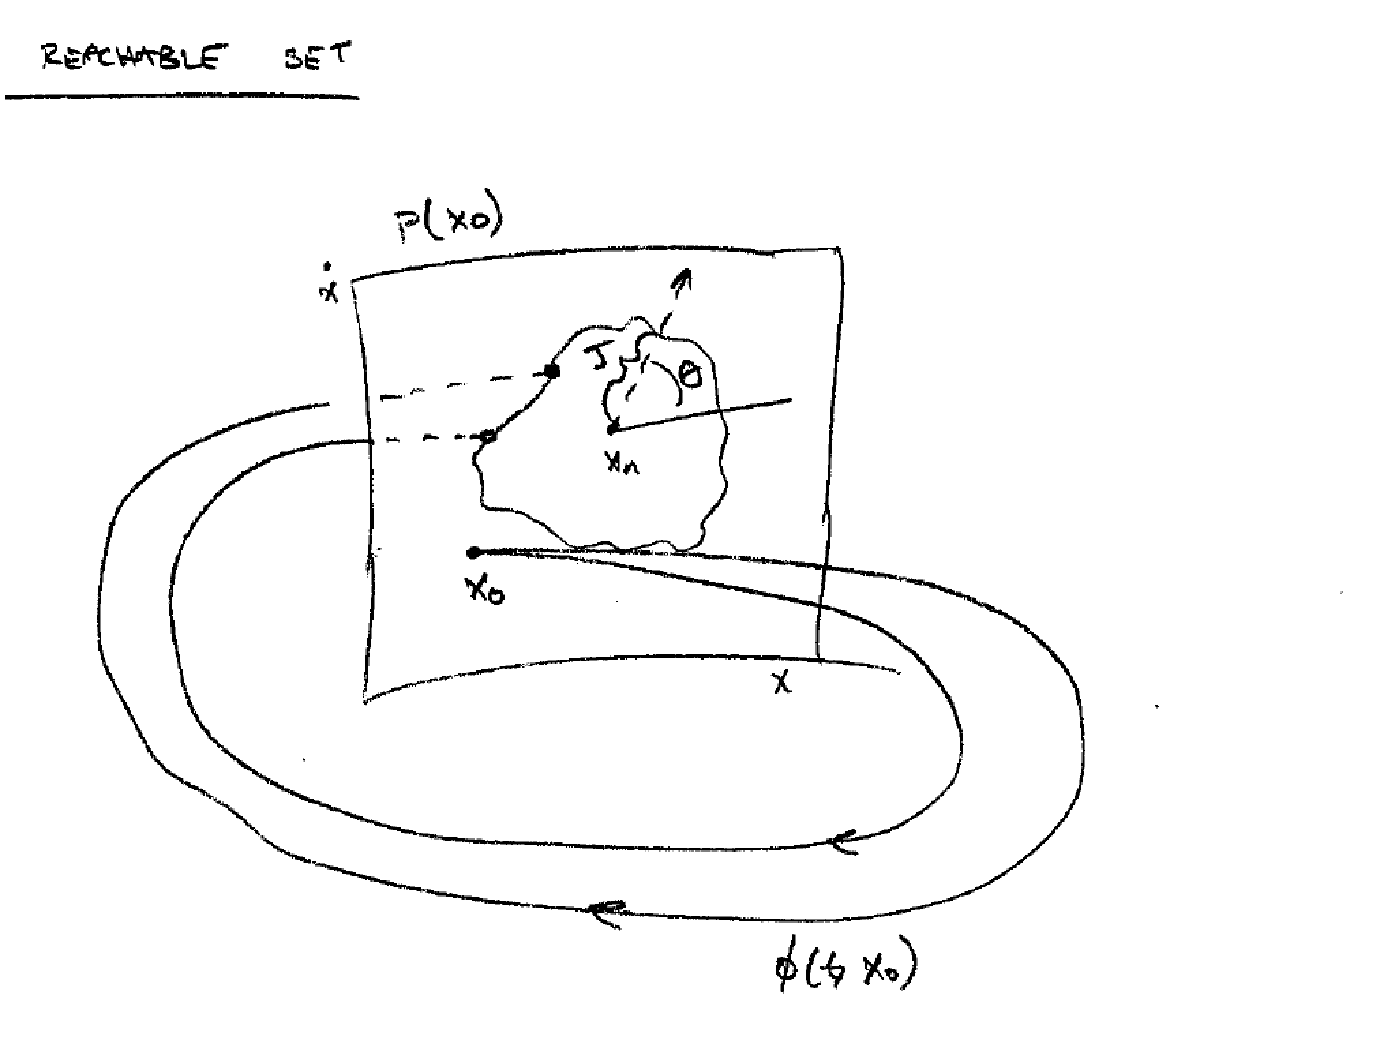
\includegraphics[width=0.5\textwidth]{reachability_set_hand}
        \begin{scaletikzpicturetowidth}{0.5\textwidth}
        \begin{tikzpicture}[tdplot_main_coords,
          poincare/.style={opacity=.2,very thick,fill=blue},
          orbit/.style={very thick,black},
          orbit hidden/.style={very thick,dashed},
          grid/.style={very thin,black},
          axis/.style={->,blue,thick},
          reachability/.style={thick,blue},scale=\tikzscale]

        % nodes for the poincare section
        \node[label=above:\(\Sigma\)] (upper_right) at (0,5,5) {};
        \node[] (upper_left) at (0,1,5) {};
        \node[] (lower_left) at (0,1,0) {};
        \node[] (lower_right) at (0,5,0) {};

        % draw poincare section
        \draw[poincare] (upper_right.center) -- (upper_left.center) -- (lower_left.center) -- (lower_right.center) -- (upper_right.center);
        
        % draw a periodic orbit
        \coordinate (center) at (0,0,2);
        \node[label=below:\(\vecbf{x}_n\)] (x0) at (0,3,2) {};
        % \node[label=below:\(\vecbf{x}_n\)] at (x0) {};
        \filldraw (x0) circle (3pt);

        % \tdplotdrawarc[orbit hidden]{(center)}{3}{90}{200}{}{};
        \tdplotdrawarc[orbit,<-]{(center)}{3}{-160}{90}{}{};

        % draw reachability set on the poincare section
        \coordinate (reach) at (0,4.5,2);
        \tdplotsetthetaplanecoords{90}

        \draw[tdplot_rotated_coords,grid] (x0) -- (reach);
        \draw[tdplot_rotated_coords,grid] (x0) -- ++(-45:1.5);

        \tdplotdrawarc[tdplot_rotated_coords,grid]{(x0)}{0.5}{-45}{90}{above}{\(\phi\)};

        % draw terminal state on reachability set
        \node[tdplot_rotated_coords,label=above:\(\vecbf{x}_f\)] (xf) at ($ (x0)+(-45:1.5) $) {};
        \filldraw (xf) circle (3pt);

        \node[tdplot_rotated_coords,label=below:\(J\)] at (xf) {};

        \tdplotdrawarc[tdplot_rotated_coords,reachability]{(x0)}{1.5}{0}{360}{}{};
        % place
    \end{tikzpicture}
        \end{scaletikzpicturetowidth}
        \caption{Reachability set on a \Poincare section\label{fig:reachability_set}}
\end{figure}

We define the \Poincare section along the horizontal axis, which is equivalent to the surface \( y = 0 \), and given by
\begin{align}
        \Sigma = \braces{ ( x, \dot{x}) \, | \, y = 0} . 
        \label{eqn:poincare_section}
\end{align}
This is similar to the previous work in determining homoclinic orbits in the three-body problem~\cite{llibre1985,koon2011}.
Previous analytical results have shown that homoclinic orbits intersect transversally in the \( (x, \dot{x} ) \) space on the plane \( y = 0 \).
We seek to compliment these results with the addition of low thrust propulsion to maximize the reachable set on the \Poincare section.
Placing our section at \( y = 0\) ensures that all trajectories will intersect our section.
An optimal control problem is defined by a  cost function
\begin{equation}
        J = -\frac{1}{2} \left( \vecbf{x}(N) - \vecbf{x}_{n}(N)\right)^T 
        \left[
        \begin{array}{cccc}
                1 & 0& 0& 0 \\
                 0& 0& 0& 0\\
                 0 & 0 & 1 &0\\
                 0 & 0& 0& 0
        \end{array}
        \right]
        \left( \vecbf{x}(N) - \vecbf{x}_{n}(N)\right) = \phi(\vecbf{x}(N),\vecbf{x}_n(N)) \, .
        \label{eq:cost}
\end{equation}
The term \( \vecbf{x}_n(N) \) is the final state of a control-free trajectory while the term \( \vecbf{x}(N)\) is the final state under the influence of the control input.
Maximization of the distance between \( \vecbf{x}_n \) and \(\vecbf{x} \), on the \Poincare section defined in~\cref{eqn:poincare_section} at the terminal time \( t_f = N \), is equivalent to the minimization of \( J \) defined in~\cref{eq:cost}.
The \Poincare section is defined through the use of appropriate terminal constraints given by
\begin{subequations}
\begin{align}
    v_1( \vecbf{x}(N) ) &= y(N) = 0 \, , \\ 
    v_2 ( \vecbf{x}(N) )&=  \frac{\dot{x}(N) - \dot{x}_n(N) }{x(N) -x_n(N) } - \tan{\theta_d} = 0\, , \\
         0 &\geq\vecbf{u}^T \vecbf{u} - u_{max}^2 \, ,
\end{align}
    \label{eq:constraints}
\end{subequations}
where the angle \( \theta_d\) defines a direction in which we wish to maximize the reachability set on the \Poincare section.
The maximum control thrust magnitude is defined by \( u_{max} \) and is non-dimensionalized by the characteristic units of length, mass, and time.
The goal is to determine the control input \( \vecbf{u}_k\) such that the cost function~\cref{eq:cost} is minimized subject to the state equations of motion~\cref{eq:discrete_eoms} and constraints~\cref{eq:constraints}.

Application of the Euler-Lagrange equations allows us to derive the necessary conditions for optimality~\cite{bryson1975}.
The discrete variational integrator in~\cref{eq:discrete_eoms} is used rather than the continuous time counterpart. 
This results in a discrete optimal control problem and the discrete necessary conditions are given as
\begin{subequations}\label{eq:necc_cond}
\begin{align}
        \vecbf{\lambda}_{k+1}^T &= \vecbf{\lambda}_k^T  \parenth{\deriv{\vecbf{f}_k}{\vecbf{x}_k}}^{-1} \, , \\
        0 &=  \deriv{H_k}{\vecbf{u}_k} \, , \label{eqn:control_necc_cond}\\
        0 &= \deriv{\phi}{\vecbf{x}_k}^T + \deriv{\vecbf{v}}{\vecbf{x}_k}^T \vecbf{\beta}  - \vecbf{\lambda}^T(N) \, ,  
\end{align}
\end{subequations}
where the Hamiltonian \(H\) is defined as
\begin{equation}
        H_k = \vecbf{\lambda}_k^T \vecbf{f}(\vecbf{x}_k, \vecbf{u}_k) \, ,
        \label{eq:hamiltonian_opt}
\end{equation}
and \( \vecbf{\lambda} \in \R^{4 \times 1} \) is the costate and \(\vecbf{\beta} \in \R^{2 \times 1} \) are the additional Lagrange multipliers associated with the terminal constraints in~\cref{eq:constraints}.
The state dynamics are represented by \( \vecbf{f}(\vecbf{x}_k, \vecbf{\lambda}_k ) \) after substituting~\cref{eqn:control_necc_cond} into~\cref{eq:discrete_eoms}.
This indirect optimal control formulation leads to a two point boundary value problem with split boundary conditions. 
By sweeping the angle \( \theta_d \) one can approximate the reachable set on the \Poincare section subject to the bounded control input. 

The costate equation of motion requires the Jacobian of~\cref{eq:discrete_eoms} and is given by
\begin{align}\label{eq:costate_eom}
        \vecbf{\lambda}_{k+1}^T = \vecbf{\lambda}_k^T
        \begin{bmatrix} 
                f_{1_x} & f_{1_y} & f_{1_{\dot{x}}} & f_{1_{\dot{y}}} \\
                f_{2_x} & f_{2_y} & f_{2_{\dot{x}}} & f_{2_{\dot{y}}} \\
                f_{3_x} & f_{3_y} & f_{3_{\dot{x}}} & f_{3_{\dot{y}}} \\
                f_{4_x} & f_{4_y} & f_{4_{\dot{x}}} & f_{4_{\dot{y}}}
        \end{bmatrix} ^ {-1} \, .
\end{align}
The derivation of~\cref{eq:costate_eom} is given in Appendix A.
In addition, the computation of~\cref{eq:costate_eom} requires inversion of the Jacobian matrix.
This is a computationally expensive operation that is prone to numerical error and instability.
We use Gauss-Jordan elimination to avoid this inversion in~\cref{eq:costate_eom} and determine an explicit update map \( \vecbf{\lambda}_k \to \vecbf{\lambda}_{k+1} \).

The optimal control formulation presented in this section results in a two point boundary value problem (TPBVP). 
There exist many methods to solve TPBVPs such as gradient, quasilinearization, and shooting methods~\cite{bryson1975,kirk2012}.
Shooting methods are common in astrodynamic trajectory design problems and relatively simple to implement.
In the shooting method, initial conditions are varied such that a terminal constraint is satisfied, similar to the way an archer modifies the bow in order to more accurately strike a target. 
Consider the vector of initial conditions, \( \vecbf{\chi} = \braces{\vecbf{x}_0, \vecbf{\lambda}_0}\), which is varied to satisfy some terminal constraints of the form \( \vecbf{G}(\vecbf{\chi}) = \braces{\vecbf{x}_t - \vecbf{x}_n} = 0 \).
The free variables at the terminal time are computed by propogation of \( \vecbf{\chi} \) over the selected time horizon. 
At the terminal time, the constraint vector is calculated and if not satisfied \( \vecbf{\chi}\) is varied.
Rather than numerical integration over the entire time interval, multiple shooting segments the interval into several smaller sub-arcs~\cite{stoer2013}.
The multiple shooting method is implemented in this paper which alleviates many of the issues associated with single shooting approaches.

\begin{figure}
        \centering
        \begin{scaletikzpicturetowidth}{1\textwidth}
                \begin{tikzpicture}[scale=\tikzscale]
                    % \draw[help lines] (0,0) grid (20,5) ; %grid

                    \node[label=west:\(\vecbf{x}\)] (x0m) at (0,5) {};
                    \node[] (x1m) at (5,5) {};
                    \node[] (x2m) at (10,5) {};
                    \node[] (x3m) at (15,5) {};
                    \node[] (xnm) at (20,5) {};

                    \node[label=below:\(k_0\)] (t0) at (0,0) {};
                    \node[label=below:\(k_1\)] (t1) at (5,0) {};
                    \node[label=below:\(k_2\)] (t2) at (10,0) {};
                    \node[label=below:\(k_{n-1}\)] (t3) at (15,0) {};
                    \node[label=below:\(k_n\)] (tn) at (20,0) {};

                    % nodes for each subsegment
                    \node[label=left:\(\vecbf{x}_0\)] (x0) at (0,1) {\pgfuseplotmark{*}};
                    \node[label=below left:\(\vecbf{\lambda}_0\)] at (x0) {};

                    \node[label=right:\(\vecbf{x}_1^{-}\)] (x1minus) at (5,2) {\pgfuseplotmark{*}};
                    \node[label=below right:\(\vecbf{\lambda}_1^{-}\)] at (x1minus) {};

                    \node[label=above left:\(\vecbf{x}_1^{+}\)] (x1plus) at (5,3) {\pgfuseplotmark{o}};
                    \node[label=left:\(\vecbf{\lambda}_1^{+}\)] at (x1plus) {};

                    \node[label=right:\(\vecbf{x}_2^{-}\)] (x2minus) at (10,2) {\pgfuseplotmark{*}};
                    \node[label=below right:\(\vecbf{\lambda}_2^{-}\)] at (x2minus) {};

                    \node[label=above left:\(\vecbf{x}_2^{+}\)] (x2plus) at (10,3) {\pgfuseplotmark{o}};
                    \node[label=left:\(\vecbf{\lambda}_2^{+}\)] at (x2plus) {};

                    \node[label=right:\(\vecbf{x}_{n-1}^{-}\)] (x3minus) at (15,2) {\pgfuseplotmark{*}};
                    \node[label=below right:\(\vecbf{\lambda}_{n-1}^{-}\)] at (x3minus) {};

                    \node[label=above left:\(\vecbf{x}_{n-1}^{+}\)] (x3plus) at (15,3) {\pgfuseplotmark{o}};
                    \node[label=left:\(\vecbf{\lambda}_{n-1}^{+}\)] at (x3plus) {};

                    \node[label=right:\(\vecbf{x}_n\)] (xnminus) at (20,3) {\pgfuseplotmark{*}};
                    \node[label=below right:\(\vecbf{\lambda}_n\)] at (xnminus) {};
                    % draw axes
                    \draw [<->,thick] (tn.center) -- (t0.center) -- (x0m.center);

                    % draw segement dividers
                    \draw [dashed,thick] (t1.center) -- (x1m.center);
                    \draw [dashed,thick] (t2.center) -- (x2m.center);
                    \draw [dashed,thick] (t3.center) -- (x3m.center);
                    \draw [dashed,thick] (tn.center) -- (xnm.center);

                    % draw markers at each subsegment

                    % draw the subsegments
                    \draw [->] (x0.center) to [bend left=30] (x1minus.center);
                    \draw [->] (x1plus.center) to [bend left=30] (x2minus.center);
                    % dotted lines here
                    \draw[decorate sep={1mm}{5mm},fill] (x2plus.east) to [bend left=10] (x3minus.west);

                    \draw [->] (x3plus.center) to [bend left=30] (xnminus.center);
                \end{tikzpicture}
        \end{scaletikzpicturetowidth}
        \caption{Multiple Shooting method\label{fig:multiple shooting}}
\end{figure}

In~\cref{fig:multiple shooting}, we show a schematic representation of the multiple shooting procedure.
We split the optimal control horizon into equal length subsegments such that the length of each segment is \( \frac{k}{n} \), where \( k, n \) are the total number of steps and number of stages, respectively.
Similarly, we divide the state and costate trajectories into \( n \) equal segments. 
To ensure continuity, additional interior constraints are incorporated as
\begin{subequations}
\begin{align}\label{eq:interior_constraints}
        \vecbf{x}_1^{-} - \vecbf{x}_1^{+} &= 0 , \\ 
        \vecbf{\lambda}_1^{-} - \vecbf{\lambda}_1^{+} &= 0 , \\
        \vecbf{x}_2^{-} - \vecbf{x}_2^{+} &= 0 , \\ 
        \vecbf{\lambda}_2^{-} - \vecbf{\lambda}_2^{+} &= 0 , \\
        &\vdots \\
        \vecbf{x}_{n-1}^{-} - \vecbf{x}_{n-1}^{+} &= 0 , \\ 
        \vecbf{\lambda}_{n-1}^{-} - \vecbf{\lambda}_{n-1}^{+} &= 0.
\end{align}
\end{subequations}
Using the multiple shooting method reduces the sensitivity of the terminal states, \( \vecbf{x}_i^{+}, \vecbf{\lambda}_i^{+}\), to variations of the initial states, \(\vecbf{x}_{i-1}^{-}, \vecbf{\lambda}_{i-1}^{-}\).
As a result, the design vector \( \vecbf{\chi} \) is augmented with the additional interior initial conditions, \( \vecbf{x}_i^{-}, \vecbf{\lambda}^{-}\).
Similarly, the constraint vector is augmented with the additional interior constraints defined in~\cref{eq:interior_constraints}.
The multiple shooting algorithm now varies the design vector \( \vecbf{\chi}\) to ensure that the constraints in \( \vecbf{G}(\vecbf{\chi}) \) are satisfied.
In this work, we use the Matlab nonlinear solver \texttt{fsolve} to solve the system of nonlinear equations defined by the multiple shooting algorithm.

% tpbvp is solved using a shooting method (fsolve in matlab)
% determine a design vector X of variables we need to determine
% define a constraint vector G(X) that we need to satisfy
% multiple shooting has interior points of continuity constraints
% sensitivity of terminal state is used to correct the initial condition (cite a book/paper)
% plot of multiple shooting ( stages)
\section{Numerical Example}\label{sec:simulation}
We present two numerical simulations in the Earth-Moon system to demonstrate the transfer procedure.
These simulations enable the spacecraft to depart from the natural dynamics through the use of low-thrust propulsion.
The reachability set on the \Poincare section allows for a straightforward method of determining transfer opportunities.
The first example is a transfer from a periodic orbit of the \( L_1 \) Lagrange point to a fixed orbit of the moon.
This example uses a single iteration of the reachable set computation in the design of the transfer.
The second example is a transfer from geostationary orbit of the Earth to a period orbit of \( L_1 \). 
This examples demonstrates the ability to extend the reachability process to multiple iterations, to allow for a much larger and more general transfer.
With both examples it is possible to depart from the vicinity of the Earth to a Moon orbit via a series of reachable sets defined on \Poincare~sections.

\subsection{Periodic Orbit transfer}\label{sec:periodic_orbit_transfer}
% define problem setup (initial and target orbits)
The first objective is to design a transfer trajectory from a planar periodic orbit about the \( L_1\) Lagrange point to a bounded orbit in the vicinity of the Moon.
The target region is created by choosing an initial condition of \( x_0 = \begin{bmatrix}1.05 & 0 & 0 & 0.35 \end{bmatrix}^T \) with \( \mu = 0.0125 \).
The target set is propagated over a period of \( t = \num{20} \) in non-dimensional units which corresponds to approximately \num{1.5} years.
\begin{figure}[htbp]
   \centering
   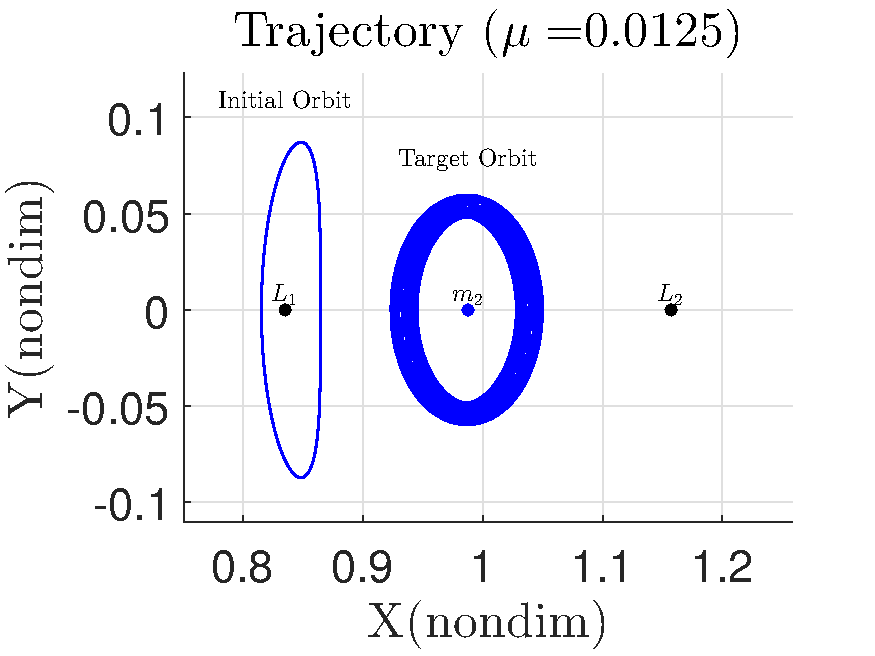
\includegraphics[width=0.5\textwidth]{moon_orbit} % requires the graphicx package
   \caption{Target Orbit Region}
   \label{fig:moon_orbit}
\end{figure}
\Cref{fig:moon_orbit} shows that the target set remains in the vicinity of the Moon, or \( m_2\), in the rotating reference frame. 
This type of orbit would be useful for a variety of mission scenarios.
For example, a series of communication satellites could be placed in this type of orbit. 
The bounded trajectories of the vehicles and constant line of sight to both the Moon and the Earth would allow for constant communication for future manned missions and potential habitats.
The initial set is a planar periodic orbit about \( L_1\), which is generated using the process of differential correction of a linear approximation~\cite{koon2011}.

% invariant manifold transfer
As a source for comparison, the method of using invariant manifolds, introduced in~\cite{koon2011}, is implemented.
As described in~\cref{sec:invariant_manifold}, these invariant manifolds are the set of trajectories that either asymptotically arrive or depart the periodic orbit. 
We generate the unstable manifold associated with the initial planar periodic orbit.
We numerically propagate the unstable manifold forward in time until the trajectories intersect the \Poincare section \( y = 0 \).
\Cref{fig:manifold_trajectory} shows the unstable invariant manifold generated from the initial \( L_1\) periodic orbit. 
The blue points in~\cref{fig:manifold_poincare} are the intersections of the target Moon orbit and the \Poincare section.
The two circular regions are the ascending (right) and descending (left) intersections of the target orbit and \Poincare section.
The green points in~\cref{fig:manifold_poincare} are intersections of the unstable manifold from~\cref{fig:manifold_trajectory} with the \Poincare section \( y = 0 \).
Only a single branch of the invariant manifold intersects with the ascending region of the target orbit.
There are no intersections of the invariant manifold with the descending region of the target orbit.
The numerical values associated with the green points denote the required time of flight along the invariant manifold in non-dimensional units.
The required travel time for a transfer using the unstable invariant manifold is  approximately \( t_f \approx 3.1\) non-dimensional time units.
\begin{figure} 
        \centering 
        \begin{subfigure}[htbp]{0.5\textwidth} 
                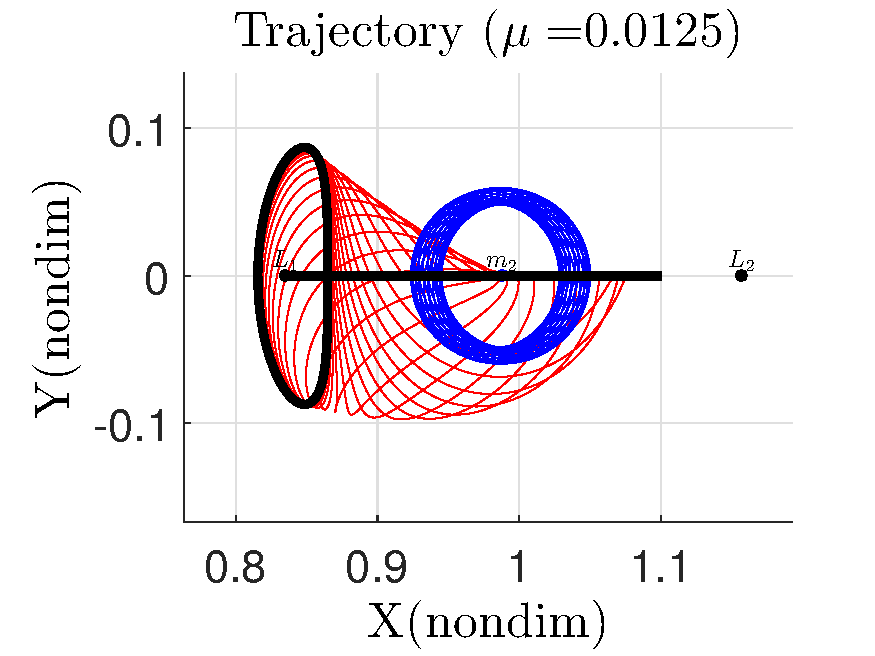
\includegraphics[width=\textwidth]{manifold_trajectory} 
                \caption{Invariant Manifold} \label{fig:manifold_trajectory} 
        \end{subfigure}~ %
        \begin{subfigure}[htbp]{0.5\textwidth} 
                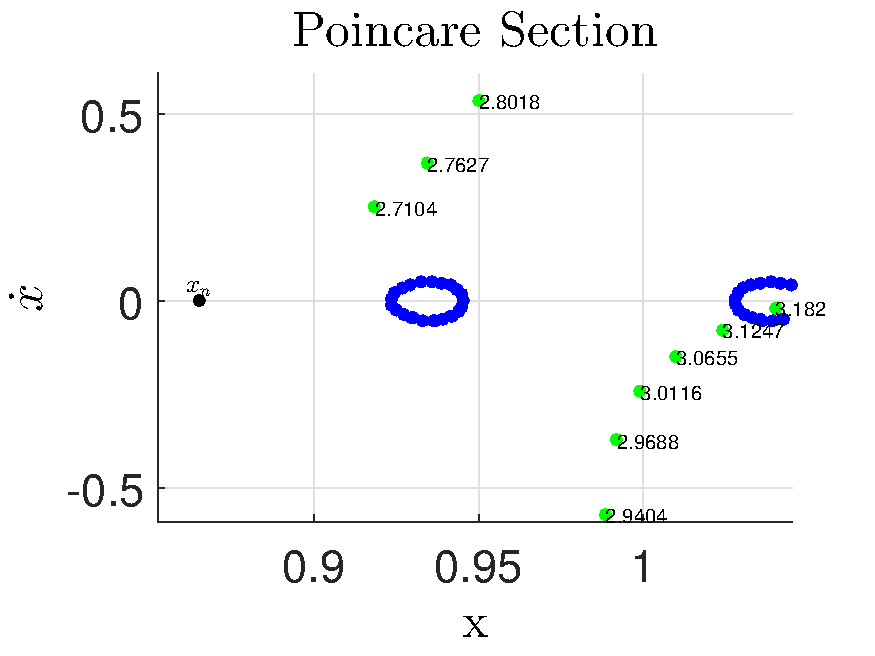
\includegraphics[width=\textwidth]{manifold_poincare} 
                \caption{Poincar\`e Section} \label{fig:manifold_poincare} 
        \end{subfigure} 
        \caption{Invariant manifold transfer}
        \label{fig:invariant_manifold_transfer} 
\end{figure}

% reachable set transfer
Next, we determine the reachability set with the addition of a low thrust control input.
We define a maximum magnitude of the thrust as \( u_{max} = 0.75 \) and assume we can point the thrust in any direction within the plane. 
This model is representative of many spacecraft which have a body fixed thruster and attitude control system.
We assume a fully actuated spacecraft model which decouples the translational and rotational dynamics.
The trajectories are generated from a fixed initial state of \( \vecbf{x}_0 = \begin{bmatrix}0.8156 & 0 & 0 & 0.1922 \end{bmatrix}^T \) over a fixed time span of \( t_f = 1.4 \).
This initial state lies on the initial periodic orbit and the time of flight is equivalent to one half period of the initial periodic orbit. 

From the initial state on the periodic orbit, a series of optimal trajectories are generated to determine the reachable set.
The multiple shooting approach is implemented to sovle the optimal control problem. 
We divide the time horizon into two equal length segments. 
The state trajectory is intialized using the free trajectory of the periodic orbit. 
Similarly, the costate trajectory is initialized from an initial guess of \( \vecbf{\lambda}_0 = \begin{bmatrix} -1 & -1 & -1 & -1\end{bmatrix}^T\) and propogated using the discrete equations of motion in~\cref{eq:costate_update}.
This results in the initial guess of the design vector \( \vecbf{\chi} = \begin{bmatrix} \vecbf{\lambda}_0 & \vecbf{x}_1^{-} & \vecbf{\lambda}_1^{-} & \vecbf{\beta} \end{bmatrix}^T\).
This design vector is then varied to ensure that the necessary conditions of optimality and the interior point constraints are satisfied. 

By varying the angle \( \theta_d\) in~\cref{eq:constraints}, a different direction along the \Poincare section is maximized. 
We discretely vary the angle over the range \( \ang{0} \leq \theta_d < \ang{360} \) to approximate the reachability set of the spacecraft.
Choosing a new angle \( \theta_d \) corresponds to a different direction as well as a new optimal control problem which is again solved using the multiple shooting approach laid out previously.
The intersection of the optimal trajectories as well as those of the target Moon orbit with the \Poincare section are shown in~\cref{fig:invariant_manifold_transfer}.

% discuss reachability set computation
The optimal trajectories, under the influence of the control input \( \vecbf{u} \), are plotted in red in~\cref{fig:reach_trajectory}.
Initially, the spacecraft is assumed to lie on the periodic orbit.
As a result, the intersection of this periodic orbit with the \Poincare section are two points corresponding to the two crossing of the orbit.
We show the control-free intersection, \( \vecbf{x}_n \), of the periodic orbit on the \Poincare section in~\cref{fig:manifold_poincare,fig:poincare_compare}
The use of the continuous low thrust propulsion expands the reachable set to region bounded by the red markers in~\cref{fig:poincare_compare}.
The reachable set is an ellipsoidal region with a major axis aligned along \( \theta \approx \ang{70} \) as compared to a fixed point without any control input.
\begin{figure} 
        \centering 
        \begin{subfigure}[htbp]{0.5\textwidth} 
                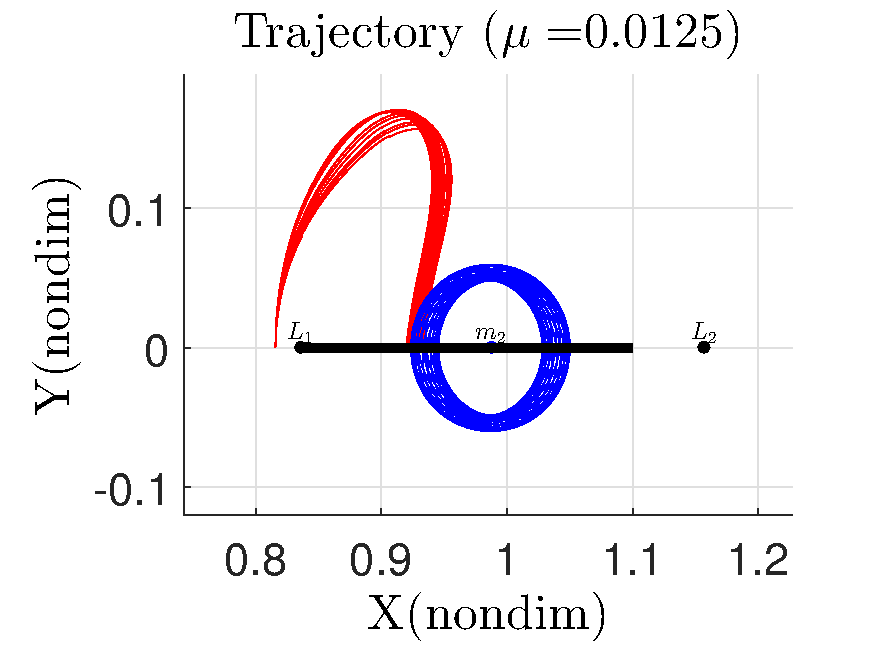
\includegraphics[width=\textwidth]{reach_trajectory} 
                \caption{Reachability set trajectories} \label{fig:reach_trajectory} 
        \end{subfigure}~ %add desired spacing between images, e. g. ~, \quad, \qquad, \hfill etc. %(or a blank line to force the subfigure onto a new line) 
        \begin{subfigure}[htbp]{0.5\textwidth} 
                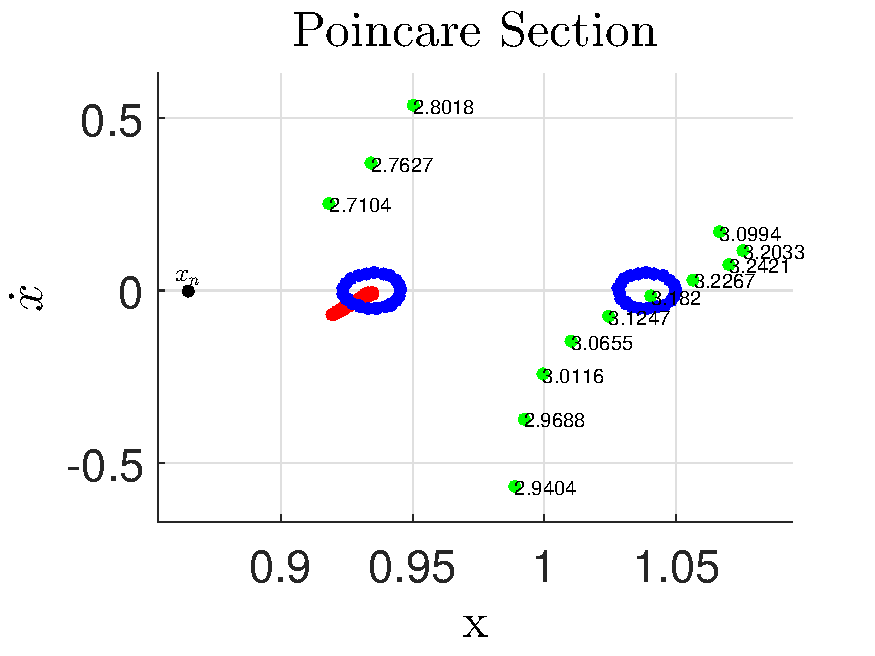
\includegraphics[width=\textwidth]{poincare_compare} 
                \caption{\Poincare section} \label{fig:poincare_compare} 
        \end{subfigure} %add desired spacing between images, e. g. ~, \quad, \qquad, \hfill etc. %(or a blank line to force the subfigure onto a new line) 
                
        \begin{subfigure}[htbp]{0.5\textwidth} 
                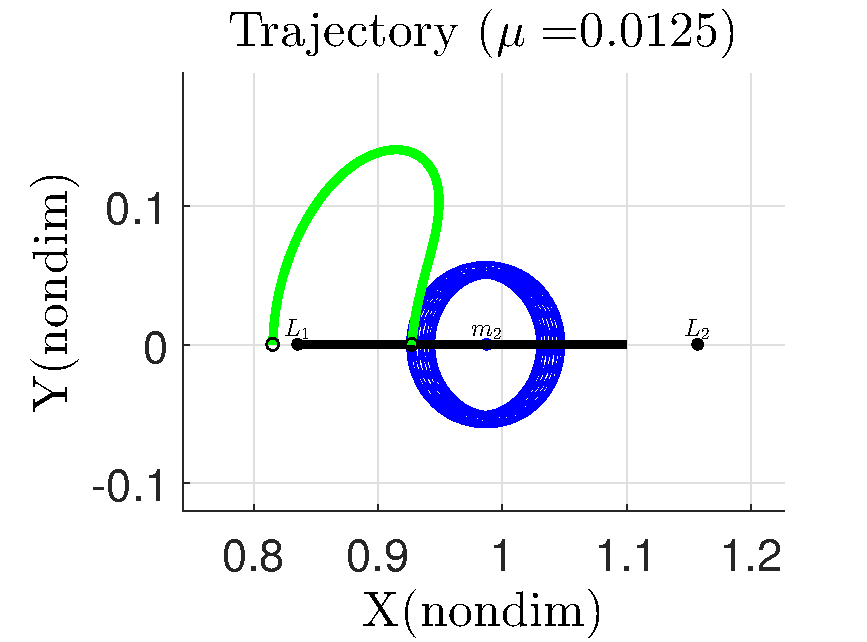
\includegraphics[width=\textwidth]{reach_transfer} 
                \caption{Final transfer trajectory} \label{fig:reach_transfer} 
        \end{subfigure}~ 
        \begin{subfigure}[htbp]{0.5\textwidth} 
                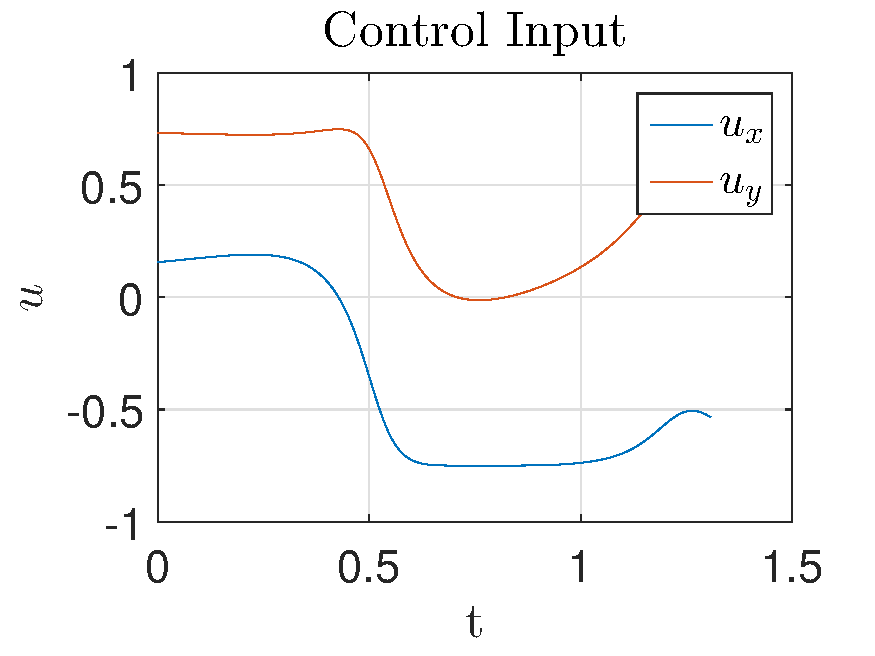
\includegraphics[width=\textwidth]{control_input_l1} 
                \caption{Control input} \label{fig:control_l1} 
        \end{subfigure}~
        \caption{Reachability set transfer}
        \label{fig:reachability_set_transfer} 
\end{figure}

% generate the optimal transfer
\Cref{fig:poincare_compare} shows that the reachable set and those of the descending target region intersect.
As both regions are discretely approximated a linear interpolation is used to determine the exact intersection state on the \Poincare section.
This intersection generates a partial target state of \( x_t \text{ and } \dot{x}_t \).
Using the energy level of the target region, defined by~\cref{eq:jacobi}, and the intersection state we can calculate the final component \( \dot{y} \) is calculated. 
This results in a complete target state \( \vecbf{x}_t \) which lies on the reachable set and on the target orbit. 
A final optimal trajectory is generated such that the \( \vecbf{x}(N) = \vecbf{x}_t \).
This transfer trajectory is denoted by the green path in~\cref{fig:reach_transfer}.
The optimal control input is shown in~\cref{fig:control_l1}. 
The spacecraft achieves the desired target while satisfying the bounded control input.

% compare the invariant manifold method and reachability set
A transfer along the invariant manifold requires on average \( t_f \approx 3.1 \) as compared to \( t_f \approx 1.4 \) for a transfer using low thrust propulsion and the reachable set.
This long time of flight is typical of transfers using invariant manifolds.
The unstable invariant manifold traverses a large region of the phase space and is dependent on the system dynamics. 
In addition, the invariant manifolds asymptotically arrive and depart from the periodic orbit. 
As a result, it may take an arbitrarily long period of time to depart from the vicinity of the periodic orbit.
In addition, only a small portion of the invariant manifold intersects with the target Moon orbit.
In contrast, the low thrust control input we are able to enlarge the reachability set from a single point to a larger ellipsoidal region in~\cref{fig:poincare_compare}.
This achieves an intersection with the target orbit with a much lower time of flight as compared to the invariant manifold method.
In addition, by generating the reachability set we are able to compute the required control input to exactly intersect the target orbit.
This avoids having to compute and accomplish a secondary impulsive manuever to transition from the invariant manifold to the target orbit.
%Since The intersection on the \Poincare section only shows that the \( x \text{ and } \dot{x} \) components intersect.
%An additional instantaneous \( \Delta V \) would be required to transfer from the invariant manifold to the target.

\subsection{Geostationary Transfer}\label{sec:geo_transfer}

% motivation - may need to compute several reachability sets
There are many situations where a more complicated and extensive orbital transfer is desired. 
For example, we present a simulation of transferring from a geostationary orbit to the a periodic orbit about the Moon.
This type of low energy transfer would be most suitable for unmanned spacecraft transitioning from the Earth to the Moon.
The long time of flight would make such a transfer unsuitable for manned missions due to life support constraints.
%This type of low energy transfer is best suited for autonomous spacecraft missions as the long time of flight is undesirable for manned spacecraft. 
Future proposals for permanent lunar spacecraft and bases will require frequent supply missions to remain viable. 
Low energy transfers from the Earth to the Lagrange points are necessary for future missions.

The previous example demonstrated the capability of determining an orbital transfer after determining the intersection of the reachability set and a target orbit.
However, it may not be possible to achieve an intersection on the \Poincare section after a single iteration. 
Since the spacecraft has an upper bounded control input and time of flight the reachability set is finite in size. 
As a result, we present a method of performing several iterations of the reachability set computation. 
A straightforward method is presented which allows for a series of reachability sets to be computed which progressively move the trajectory towards the target.
In this manner, it is possible to determine more complicated transfers by a simple selection of states from the reachability set.

% discuss difficulties in applying direct optimization or the invariant manifold method
It is possible to design arbitrary transfers using either a direct optimization or invariant manifold based approach.
The direct optimization method transforms the optimal control problem into a nonlinear programming problem.
Instead of solving the Euler-Lagrange equations the state and control histories are parameterized and solved through any number of mathematical programming methods.
However, due to this parameterization only an approximate solution, which approximates the true optimal solution in the limit, is feasible. 
On the other hand, our method applies an indirect optimization method.
The necessary conditions for optimality are computed and directly solved in generating the reachability set. 
The use of the reachability set also avoids the issues of selecting a valid initial condition.
We select a state on the maximum reachability set which minimizes the distance toward the target. 
This straightforward approach achieves an optimal trajectory and is used to generate general transfers.

The invariant manifold method is difficult to apply to general orbital transfers. 
The manifolds are associated with periodic orbits in the three-body system. 
In this case, an appropriate periodic orbit must first be determined prior to generating the invariant manifold.
Furthermore, there is no guarantee that the invariant manifold will pass through a desired region of space. 
For example, in the Earth-Moon system the unstable manifolds of periodic orbits about \( L_1 \) do not pass close to the Earth, but rather are beyond the geostationary orbit altitude. 
In addition, determining the intersections between various invariant manifolds is not trivial. 
It requires an appropriate \Poincare section and the generation of several invariant manifolds.
There is no clear method of selecting the periodic orbits required based on a the type of transfer desired. 
Determining an intersection between these invariant manifolds generally requires extended flight times, involving several orbits of the primaries, before an appropriate intersection is found.
As a result, it is difficult to generalize this method to arbitrary transfers in the three-body problem.

% describe initial and target states for this example
This numerical simulation demonstrates the ability of the proposed approach. 
We use multiple iterations of the reachability set to achieve a more complicated transfer.
In this manner, it is possible to design arbitrary transfers which are not possible using a single reachability computation.
Initially, it is assumed that the spacecraft lies on a circular geostationary orbit in the non-dimensional Earth-Moon three-body system. 
The geostationary orbit about the Earth is transformed into the rotating reference frame of the Earth-Moon three body problem.
In addition, we nondimensionalize the initial state to find \( \vecbf{x}_0 = \begin{bmatrix} 0.0972 & 0 & 0 & 3.0010\end{bmatrix}^T\) as the initial condition of the spacecraft on the geostationary orbit.
It is desired to transfer to a periodic orbit about the \( L_1 \) Lagrange point. 
The periodic orbit is defined by the initial condition \(\begin{bmatrix} 0.8057 & 0 & 0 & 0.2982 \end{bmatrix} \).
The initial and target orbits are illustrated in~\cref{fig:geo_transfer_target}.
\begin{figure}[htbp]
   \centering
   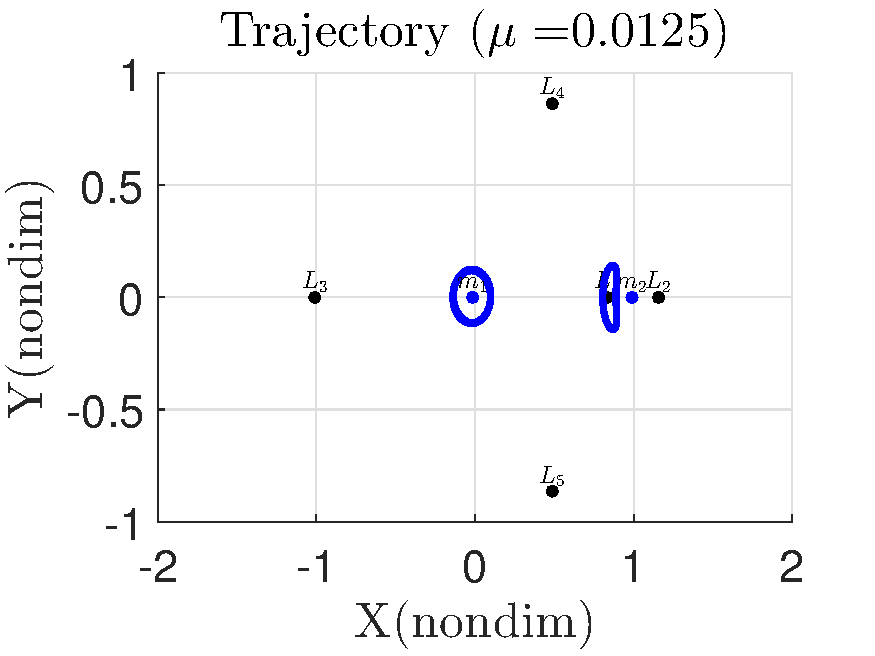
\includegraphics[width=0.5\textwidth]{initial_final} % requires the graphicx package
   \caption{Transfer target}
   \label{fig:geo_transfer_target}
\end{figure}
In order to effectively utilize the dynamics of the three-body system the stable manifold of the periodic orbit is targeted.
We seek to generate a transfer from the geostationary orbit onto the stable invariant manfiold.
Once on the manifold, the spacecraft will coast in an uncontrolled fashion and asymptotically arrive at the desired periodic orbit.

\begin{figure}[htbp]
   \centering
   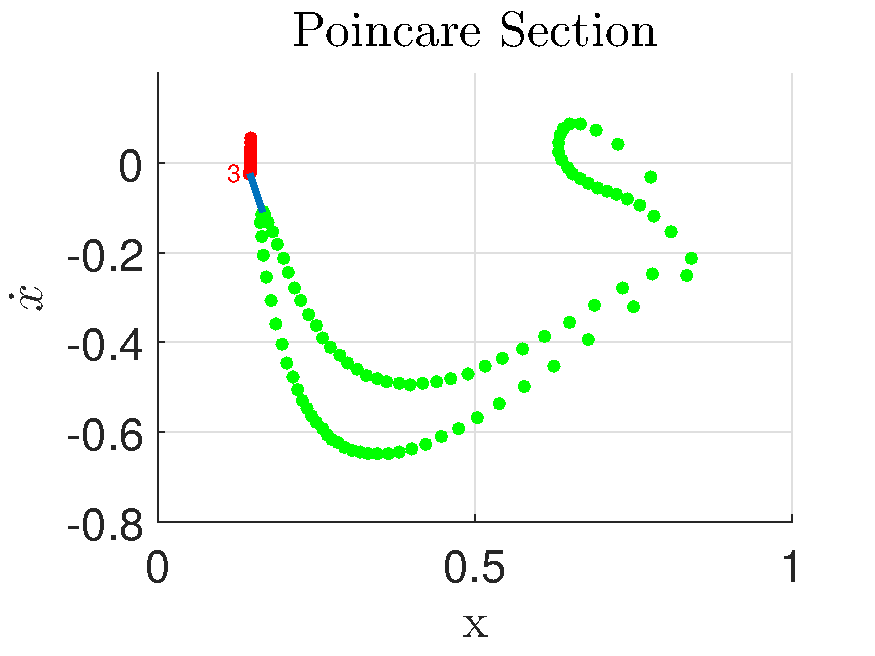
\includegraphics[width=0.5\textwidth]{third_reachability_set} % requires the graphicx package
   \caption{Reachable set after three iterations}
   \label{fig:third_reachability_set}
\end{figure}
Next, we generate the stable invariant manifold associated with the periodic orbit in order to determine our target set.
The stable manifold is propagated to the \Poincare section at \( y = 0 \), which is denoted by the horizontal black line in~\cref{fig:geo_transfer_full}.
Next, we compute the reachable sets originating on the geo-stationary orbit and subject to the maximum control constraint. 
The multiple shooting approach is used to solve the optimal control problem with two segments.
For the first reachability set computation, the initial geostationary orbit is used to initialize the multiple shooting algorithm.
We use the same initial guess of \( \vecbf{\lambda}_0\) as in~\cref{sec:periodic_orbit_transfer} and propogate over the fixed time horizon of the period of the geostationary orbit to initialize \( \vecbf{\lambda}_i^{-}\).

The first reachable set is computed beginning on the geostationary orbit at it's intersection with the \Poincare section and we again assume a upper bound on the thrust magnitude of \( u_{max} = 0.75 \).
The reachable set is generated by varying the angle \( \ang{0} \leq \theta < \ang{360} \) in~\cref{eq:constraints} defined on the \Poincare section.
This allows us to approximate the set of states that are achievable in the \( \parenth{x ,\dot{x}} \) space.
After each computation of the reachability set we pick a state which minimizes the distance on the \Poincare section towards the stable manifolds as the function \( d \)
\begin{align*}
        d(\vecbf{x}(N)) = \sqrt{\parenth{x - x_t}^2 + \parenth{\dot{x} - \dot{x}_t}^2}.
\end{align*}
From the reachable set, the trajectory which minimizes \( d \) is used to intialize the next iteration.
Once the reachability set intersects the stable manifold, we can achieve a complete transfer from the initial geostationary orbit to the stable manifold of \( L_1 \).
%A state is chosen from the reachable set which minimizes the distance on the \Poincare section to the stable manifold, illustrated in green in~\cref{fig:geo_transfer_poincare}, and is used as the initial condition for the next reachable set computation.
For example,~\cref{fig:third_reachability_set} shows the reachable set after three iterations in red and the minimum distance to the stable manifold in green.
The state and costate trajectories associated with this point on the rechable set is used to initialize the following iteration. 
In this manner, the multiple shooting algorithm solves the optimal control problem and generates reachable sets which move away from the intial orbit and towards the desired target.

With each reachable set we move the controlled trajectory closer to the target stable manifold.
\Cref{fig:geo_transfer_poincare} shows that after eight iterations the resulting trajectory intersects the stable manifold. 
Combining these trajectories results in the powered portion of the transfer from the geostationary orbit to the stable manifold. 
\Cref{fig:geo_transfer_full,fig:geo_transfer_zoom} shows the resulting trajectory, with the final trajectory shown in red which ensures the intersection with the stable invariant manifold.
Once at the stable manifold, no further control input is required and the vehicle will coast towards the target periodic orbit.
\Cref{fig:control_input_geo} shows the control input during the powered portion of the transfer. 
The spacecraft maintains a bounded control magnitude during the transfer to the stable manifold.
\begin{figure} 
        \centering 
        \begin{subfigure}[htbp]{0.5\textwidth} 
                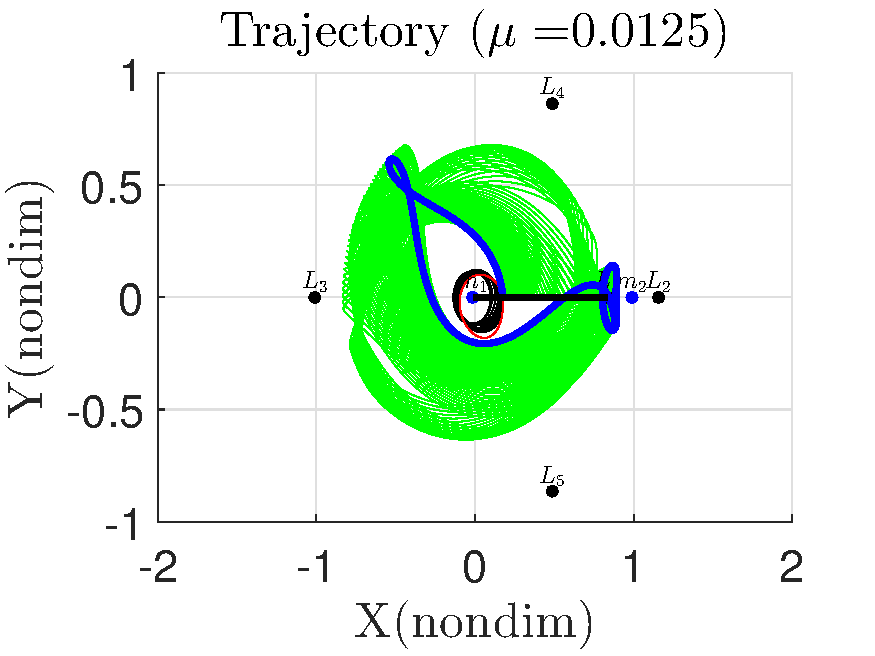
\includegraphics[width=\textwidth]{geo_transfer_full} 
                \caption{Completed transfer trajectory} \label{fig:geo_transfer_full} 
        \end{subfigure}~ %add desired spacing between images, e. g. ~, \quad, \qquad, \hfill etc. %(or a blank line to force the subfigure onto a new line) 
        \begin{subfigure}[htbp]{0.5\textwidth} 
                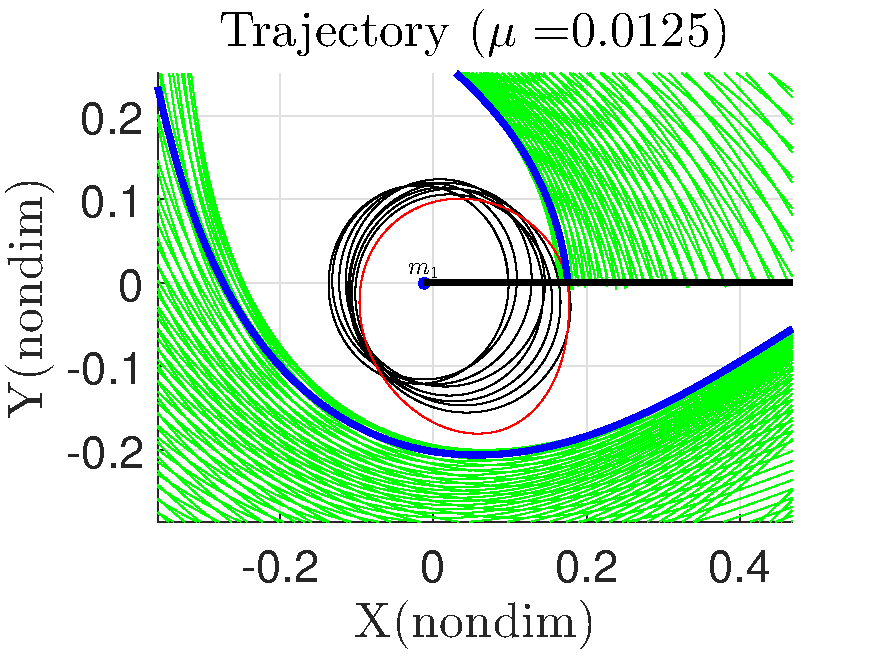
\includegraphics[width=\textwidth]{geo_transfer_zoom} 
                \caption{Detailed view of transfer} \label{fig:geo_transfer_zoom} 
        \end{subfigure} 
        
        \begin{subfigure}[htbp]{0.5\textwidth} 
                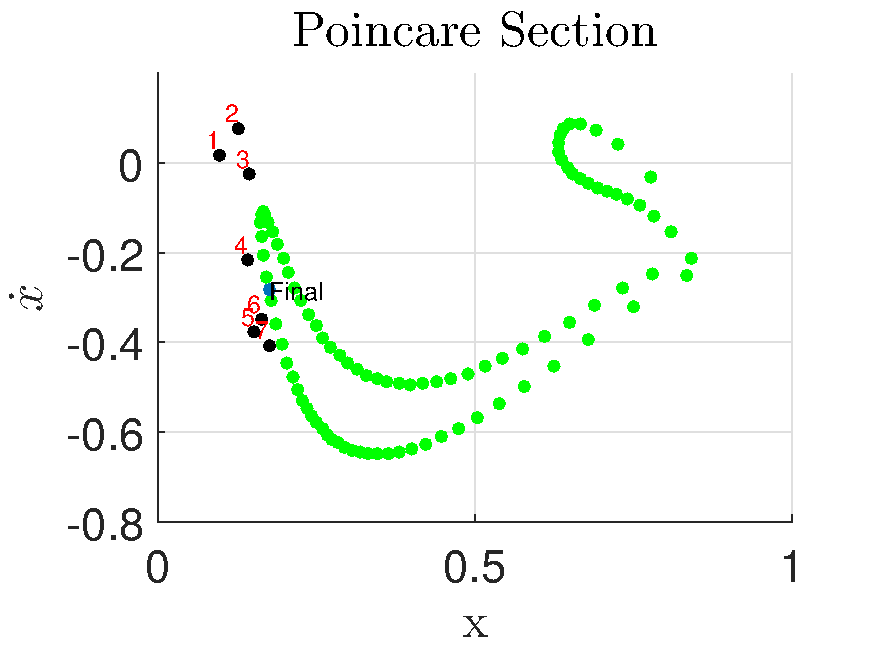
\includegraphics[width=\textwidth]{poincare} 
                \caption{\Poincare section} \label{fig:geo_transfer_poincare} 
        \end{subfigure}~%
        \begin{subfigure}[htbp]{0.5\textwidth} 
                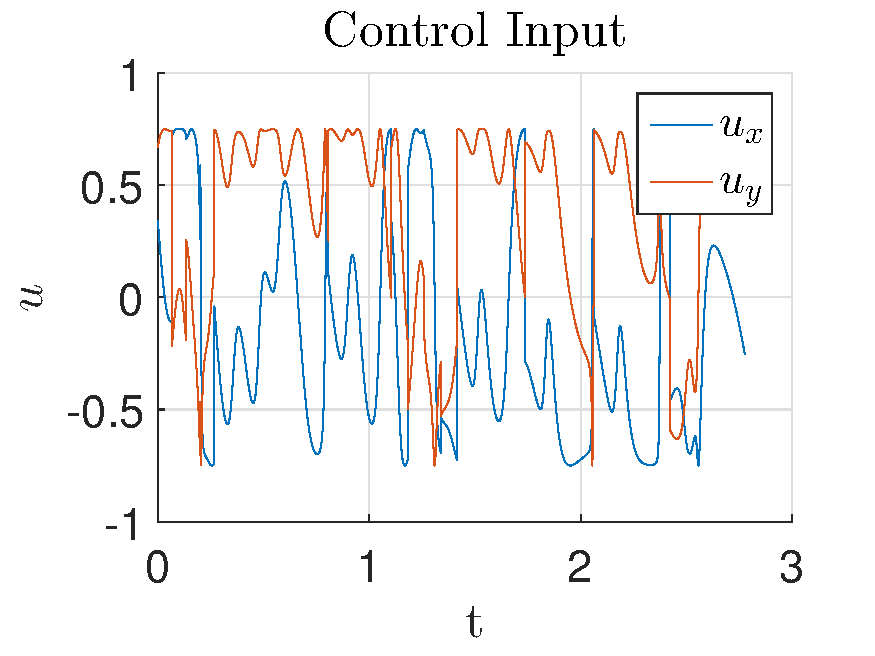
\includegraphics[width=\textwidth]{control_input_geo} 
                \caption{Control input} \label{fig:control_input_geo} 
        \end{subfigure} 
        \caption{Transfer from geostationary orbit to the \( L_1 \) stable manifold using multiple iterations of the reachability set}
        \label{fig:geo_transfer} 
\end{figure}

This approach demonstrates the ability to link several computations of the reachability set to enable a more general transfer.
We use eight iterations in order to transfer from the geostationary orbit to the stable manifold.
This approach allows for a larger class of potential transfers which leverage the capabilities of low-thrust propulsion systems.
We are able to achieve a transfer that is not possible via the standard invariant manifold approach. 
In addition, this example illustrates a straightforward method to depart from the natural dynamics and transfer to a large region of the phase space that is not accessible via invariant manifolds alone.

\section{Conclusions}\label{sec:conclusion}
In this paper, an optimal transfer process which combines concepts of reachability and \Poincare section is used to generate transfer between planar periodic orbits in the three-body problem.
The \Poincare section allows for trajectory design on a lower dimensional phase space and simplifies the process.
The indirect optimal control formulation enables straightforward method of incorporating additional path and control constraints.
However, the use of optimal control techniques leads to open loop trajectories that are not robust to model uncertainties or disturbances.
Lyapunov control theory, which has previously been applied to the two-body problem, is being investigated in the hope of designing closed loop control schemes for this three-body scenario~\cite{chang2002}.
This analysis has also assumed perfect attitude control and the ability to orient thrust in any direction.
The addition of attitude dynamics and realistic pointing constraints would significantly improve the applicability.

\appendix
\section*{Appendix A: Costate Equations of Motion}\label{sec:costate_appendix}
The development of the costate equations of motions begins with determining the second order partial derivatives of the gravitational potential. 
Due to the symmetry of partial derivatives only three terms are required and are given by
\begin{align}\label{eq:second_discrete_potential_grad}
        U_{x\xk} &= \parenth{1-\mu} \bracket{\frac{1}{\distonek^3} - \frac{3 \parenth{\xk +\mu}^2}{\distonek^5}} + \mu \bracket{\frac{1}{\disttwok^3} - \frac{3 \parenth{\xk -1 + \mu}^2}{\disttwok^5}} \, ,\\
        U_{y\yk} &= \parenth{1-\mu} \bracket{\frac{1}{\distonek^3} - \frac{3 \yk^2}{\distonek^5}} + \mu \bracket{\frac{1}{\disttwok^3} - \frac{3 \yk^2}{\disttwok^5}} \, ,\\
        U_{x\yk} &= U_{y\xk} =  \frac{-3 \parenth{1-\mu} \parenth{\xk +\mu} \yk}{\distonek^3} - \frac{3\mu\yk\parenth{\xk-1+\mu}}{\disttwok^5} \, .
\end{align}
The gradient of~\cref{eq:xkp} is given as
\begin{subequations}\label{eq:xkp_grad}
\begin{align}
        f_{1_x} &= \frac{1}{1+h^2} \bracket{h^2 + 1 + \frac{h^2}{2} -\frac{h^3}{2} U_{y\xk} - \frac{h^2}{2}U_{x\xk}} \, ,\\
        f_{1_y} &= \frac{1}{1+h^2} \bracket{ \frac{h^3}{2} -\frac{h^3}{2} U_{y\yk} - \frac{h^2}{2}U_{x\yk}} \, ,\\
        f_{1_{\dot{x}}} &= \frac{h}{1+h^2} \, ,\\
        f_{1_{\dot{y}}} &= \frac{h^2}{1+h^2} \, .
\end{align}
\end{subequations}
The gradient of~\cref{eq:ykp} is given as
\begin{subequations}\label{eq:ykp_grad}
\begin{align}
        f_{2_x} &= h -h f_{1_x} - \frac{h^2}{2} U_{y\xk} \, , \\
        f_{2_y} &= -h f_{1_y} + 1 + \frac{h^2}{2} - \frac{h^2}{2} U_{y\yk} \, ,\\
        f_{2_{\dot{x}}} &= -h f_{1_{\dot{x}}} \, ,\\
        f_{2_{\dot{y}}} &= h - h f_{1_{\dot{y}}} \, .
\end{align}
\end{subequations}
The gradients of~\cref{eq:distonekp,eq:disttwokp} are given as
\begin{subequations}\label{eq:distkp_grad}
\begin{align}
        \deriv{\distonekp}{\bar{x}} &= \parenth{\left( \xkp + \mu\right)^2 + \ykp^2}^{-\frac{1}{2}} \bracket{\parenth{\xkp + \mu} f_{1_{\bar{x}}} + \ykp f_{2_{\bar{x}}}} \, ,\\
        \deriv{\disttwokp}{\bar{x}} &= \parenth{\left( \xkp - 1 + \mu\right)^2 + \ykp^2}^{-\frac{1}{2}} \bracket{\parenth{\xkp -1 + \mu} f_{1_{\bar{x}}} + \ykp f_{2_{\bar{x}}}}  \, .
\end{align}
\end{subequations}
The second order partial derivatives of the gravitational potential at \( k+1\) are given as
\begin{subequations}
\begin{align}
        \deriv{U_{x\xkp}}{\bar{x}} &= \parenth{1-\mu}\bracket{\frac{1}{\distonekp^3} f_{1_{\bar{x}}} - \frac{3 \parenth{\xkp +mu}}{\distonekp^4} \deriv{\distonekp}{\bar{x}}} + \mu \bracket{\frac{1}{\disttwokp^3} f_{1_{\bar{x}}} - \frac{-3 \parenth{\xkp -1 + \mu}}{\disttwokp^4} \deriv{\disttwokp}{\bar{x}}} \, ,\\
        \deriv{U_{y\xkp}}{\bar{x}} &= \parenth{1-\mu}\bracket{\frac{1}{\distonekp^3} f_{2_{\bar{x}}} - \frac{3 \ykp}{\distonekp^4} \deriv{\distonekp}{\bar{x}}} + \mu \bracket{\frac{1}{\disttwokp^3} f_{2_{\bar{x}}} - \frac{-3 \ykp}{\disttwokp^4} \deriv{\disttwokp}{\bar{x}}} \, .
\end{align}
\end{subequations}
The gradient of~\cref{eq:xdotkp,eq:ydotkp} are given as
\begin{subequations}\label{eq:xdotkp_grad}
\begin{align}
        f_{3_x} &= 2 f_{2_x} + \frac{h}{2} \parenth{f_{1_x} + 1} - \frac{h}{2} U_{x\xkp} - \frac{h}{2} U_{x\xk} \, ,\\
        f_{3_y} &= -2 + 2 f_{2_y} + \frac{h}{2} f_{1_y} - \frac{h}{2} U_{x\ykp} -\frac{h}{2} U_{x\yk} \, ,\\
        f_{3_{\dot{x}}} &= 1 + 2 f_{2_{\dot{x}}} + \frac{h}{2} f_{1_{\dot{x}}} - \frac{h}{2} U_{x\xdotkp}\, ,\\
        f_{3_{\dot{y}}} &= 2 f_{2_{\dot{y}}}\, ,
\end{align}
\end{subequations}
\begin{subequations}\label{eq:ydotkp_grad}
\begin{align}
        f_{4_x} &= 2 - 2 f_{1_x} + \frac{h}{2} f_{2_x}  - \frac{h}{2} U_{y\xkp} - \frac{h}{2} U_{y\xk} \, ,\\
        f_{4_y} &= -2f_{1_y}  - \frac{h}{2} \parenth{f_{2_y} + 1} - \frac{h}{2} U_{y\ykp} -\frac{h}{2} U_{y\yk} \, ,\\
        f_{4_{\dot{x}}} &= - 2 f_{1_{\dot{x}}} +  \frac{h}{2} f_{2_{\dot{x}}} - \frac{h}{2} U_{y\xdotkp}\, ,\\
        f_{4_{\dot{y}}} &= 1 - 2 f_{1_{\dot{y}}} + \frac{h}{2} f_{2_{\dot{y}}} - \frac{h}{2} U_{y\ydotkp}\, .
\end{align}
\end{subequations}
These gradient equations are in a cascade type structure.
\Cref{eq:ydotkp_grad,eq:xdotkp_grad} are functions of~\cref{eq:xdotkp,eq:ydotkp}.
As a result, the accuracy of the Jacobian will tend to decrease as the first order approximation errors accumulate.

%\begin{acknowledgements}
%If you'd like to thank anyone, place your comments here
%and remove the percent signs.
%\end{acknowledgements}

\bibliography{library}
\bibliographystyle{spmpsci}
\end{document}
